% !TEX root = ../../thesis.tex
\chapter{Elliptic Curves\label{ch:ec}}

In this chapter, we will as briefly as possible cover the core background of elliptic curves that one needs to understand the main result and follow the references therein. We do not assume much familiarity with elliptic curves. We do assume the reader is familiar with Algebra and Algebraic Geometry, along with at least passing knowledge of some Number Theory. The primary reference used here is  standard reference for elliptic curves, namely \cite{silvermanarithmetic}. Though we have diverged from the presentation in \cite{silvermanarithmetic} whenever necessary. Throughout, unless otherwise specified, all fields will be characteristic 0. We will not discuss elliptic curves over finite, local, or function fields here. Should the reader want to go further (and there is a vast ocean we have ignored), one can see \cite{silvermanarithmetic} or any number of other common references on the topic: \cite{silvermanrational}, \cite{washington03}, \cite{knapp92}, \cite{milne06}, etc. The author particularly recommends \cite{husemoller04} for its readability. 





% Elliptic Curves & the Group Law
\section{The Group Law \& Weierstrass Equations\label{sec:equations}}

Suppose we begin with a smooth homogenous polynomial of degree 3 over a field $K$ with a $K$-rational point. We write $F(X,Y,Z)$ as in \eqref{eqn:homog1} and examine the curve defined by $F(X,Y,Z)= 0$. Note that any smooth cubic curve with a $K$-rational point can be put into this form via homogenization. Call the given $K$-rational point $P$. 
	\begin{equation} \label{eqn:homog1}
	\begin{aligned}
	F(X,Y,Z):= aX^3 + bX^2YZ + cXY^2 + dY^3 + eX^2Z  \\
	+fXYZ +gY^2Z + hXZ^2 + iYZ^2 + jZ^3,
	\end{aligned}
	\end{equation}
Because $F(X,Y,Z)$ is smooth, we can form the tangent line to $F$ at $P$. Now choose coordinates so that this tangent line is $Z= 0$. By B\'ezout's Theorem, c.f. Theorem~\ref{thm:bezout}, we know that this new line $Z= 0$ intersects the curve at another point, say $Q$. Again because the curve is smooth, we can form the tangent line to the curve at $Q$, and choose coordinates so that this tangent line is $X= 0$. Finally, choose any line through $P$ distinct from the tangent line at $P$, and choose coordinates so that this is $Y= 0$. With this new coordinate system, we have a curve $F'(X,Y,Z)= 0$ given by a smooth homogenous polynomial of degree 3 containing $P= [1,0,0]$ and $Q= [0,1,0]$. Routine verification checks that we have 
	\[
	F'(X,Y,Z):= rXY^2 + s Z \phi(X,Y,Z),
	\]
where $\phi(X,Y,Z)$ is a homogenous polynomial of degree 2. Dehomogenizing the curve, we have a smooth cubic curve
	\begin{equation} \label{eqn:homog2}
	f(x,y):= xy^2 + ax^2 + bxy + cy^2 + dx + ey + g= 0,
	\end{equation}
where the $a, b, c, d, e, g$ in \eqref{eqn:homog2} are not necessarily those in \eqref{eqn:homog1}. By abuse of notation, make the change of variables $x:= x + c$ to obtain an equation
	\[
	xy^2 + (ax + b)y= cx^2 + dx + e,
	\]
for a possibly new set of $a, b, c, d, e$. Multiplying by $x$, we have
	\[
	(xy)^2 + (ax + b)xy= cx^3 + dx^2 + ex.
	\]
Again by abuse of notation, make the change of variables $y:= yx$ followed by $y:= y - \frac{1}{2} (ax + b)$ to obtain an equation of the form $y^2= f(x)$, where $f(x)$ is a cubic polynomial in $x$ (not necessarily monic). Say that $\alpha$ is the leading coefficient of $f(x)$. As one final abuse of the notation, after making the change of variables $x:= x/\alpha$ and $y:= y/\alpha^2$, we obtain an equation
	\[
	y^2= x^3 + ax^2 + bx + c
	\]
for some $a, b, c \in K$. If one desires, making the substitution $x:= x - \alpha$ (for some carefully chosen $\alpha \in K$) eliminates the $x^2$-term to obtain $y^2= x^3 + Ax + B$, which will be an elliptic curve (in short Weierstrass form). Given that we have studied linear and quadratic (homogeneous) polynomial equations, homogeneous cubic polynomial equations was the next natural step, and we see that this is the same as studying a polynomial $y^2= x^3 + Ax + B$, which will be one of the many equivalent definitions for an elliptic curve. 


\begin{dfn}
An elliptic curve defined over a field $K$, denoted $E/K$, is any of the following equivalent objects: \leavevmode\vspace{-1em}
	\begin{enumerate}[(i)] \itemsep-1em
	\item A smooth projective curve of genus 1 over $K$ with a distinguished $K$-rational point.
	\item The set $\{ (x,y) \colon y^2 + a_1xy + a_3y= x^3 + a_2x^2 + a_4x + a_6, \Delta_E \neq 0 \} \cup \{ \infty \}$ with an addition structure given by the Chord-Tangent Law. 
	\item The set $\{ (x,y) \colon y^2= x^3 + Ax + B, -16(4A^3 + 27B^2) \neq 0 \} \cup \{ \infty \}$ with an addition structure given by the Chord-Tangent Law. 
	\item A compact Riemann surface of genus 1. 
	\item An abelian variety of dimension 1 over $K$.
	\end{enumerate}
\end{dfn}


We will only briefly describe how these definitions are equivalent. For any thorough discussion of these equivalencies, see any ``standard'' elliptic curve reference, e.g. \cite{husemoller04}, \cite{silvermanarithmetic}, \cite{washington03}, \cite{knapp92}, \cite{milne06}, etc. Before discussing the addition law on an elliptic curve, we examine their ``set structure.'' We begin with the equation in (ii), called the (general) Weierstrass form of an elliptic curve:
	\[
	y^2 + a_1xy + a_3y= x^3 + a_2x^2 + a_4x + a_6.
	\]
Denote by $\{ \infty \}$ the point at infinity, $\cO:= [0,1,0]$. If $\ch \ov{K} \neq 2$, we can complete the square by making the substitution
	\[
	y \mapsto \dfrac{1}{2} (y - a_1x - a_3),
	\]
which gives an equation of the form $y^2= 4x^3 + b_2x^2 + 2b_4x + b_6$, where $b_2= a_1^2 + 4a_2$, $b_4= 2a_4 + a_1a_3$, $b_6= a_3^2 + 4a_5$. Define
	\[
	\begin{aligned}
	b_8&= a_1^2a_6 + 4a_2a_6 - a_1a_3a_4 + a_2a_3^2 - a_4^2 &\quad&& \Delta_E&= -b_2^2b_8 - 8b_4^3 - 27b_6^2 + 9b_2b_4b_6 \\
	c_4&= b_2^2 - 24b_4 &&& j&= \dfrac{c_4^3}{\Delta_E} \\
	c_6&= -b_2^3 + 36b_2b_4 - 216b_6 &&& \omega&= \dfrac{dx}{2y + a_1x + a_3}= \dfrac{dy}{3x^2 + 2a_2x + a_4 - a_1y}.
	\end{aligned}
	\]
We call $\Delta_E$, or just $\Delta$, the discriminant of $E$, $j$ the $j$-invariant of $E$, and $\omega$ the invariant differential associated to the equation for $E$. It is routine to verify that $4b_8= b_2b_6 - b_4^2$ and $1728\Delta= c_4^3 - c_6^2$. Assume also that $\ch \ov{K} \neq 2, 3$. Then we can make the substitution
	\[
	(x,y) \mapsto \left( \dfrac{x - 3b_2}{36}, \dfrac{y}{108} \right),
	\]
which eliminates the $x^2$ term, so that we obtain $y^2= x^3 - 27c_4x - 54c_6$---which is also referred to as the (short) Weierstrass form for $E$. Of course, there are many different equations that give the same elliptic curve. However, if one assumes that the line $Z= 0$ in projective space intersects $E$ only at $\cO$, the only change of variables fixing $\cO$ and preserving the Weierstrass form is $x= u^2x' + r$ and $y= u^3y' + u^2sx' + t$, where $u,r,s,t \in \ov{K}$ and $u \neq 0$. One can compute the new $a$'s one obtains after such a substitution:
	\[
	\begin{aligned}
	ua_1'&= a_1 + 2s & u^6b_6'&= b_6 + 2rb_4 + r^2b_2 + 4r^3 \\
	u^2a_2'&= a_2 - sa_1 + 3r - s^2 & u^8b_8'&= b_8 + 3rb_6 + 3r^2b_4 + r^3b_2 + 3r^4 \\
	u^3a_3'&= a_3 + ra_1 + 2t & u^4c_4'&= c_4 \\
	u^4a_4'&= a_4 - sa_3 + 2ra_2 - (t + rs)a_1 + 3r^2 - 2st & u^6c_6'&= c_6 \\
	u^6a_6'&= a_6 + ra_4 + r^2a_2 + r^3 - ta_3 - t^2 - rta_1 & u^{12}\Delta'&= \Delta \\
	u^2b_2'&= b_2 + 12r & j'&= j \\
	u^4b_4'&= b_4 + rb_2 + 6r^2 & u^{-1}\omega'&= \omega.
	\end{aligned}
	\]
For more on all this, see \cite[III.1]{silvermanarithmetic}. Take note that after such a substitution, $\Delta$ differs from $\Delta'$ by a square in $K$. 


\begin{prop}[{\cite[III.1, Prop.~1.4]{silvermanarithmetic}}] \hfill
\leavevmode\vspace{-1em}
        \begin{enumerate}[(a)] \itemsep-1em
        \item The curve given by a Weierstrass equation satisfies: \leavevmode\vspace{-1em}
            	\begin{enumerate}[(i)] \itemsep-1em
            	\item It is nonsingular if and only if $\Delta \neq 0$.
            	\item It has a node if and only if $\Delta= 0$ and $c_4 \neq 0$.
            	\item It has a cusp if and only if $\Delta= c_4= 0$.\leavevmode\vspace{-1em}
            	\end{enumerate} 
        In cases (ii) and (iii), there is only one singular point. 
        \item Two elliptic curves are isomorphic over $\ov{K}$ if and only if they both have the same $j$-invariant. 
        
        \item Let $j_0 \in \ov{K}$. There exists an elliptic curve defined over $K(j_0)$ whose $j$-invariant is equal to $j_0$. 
        \end{enumerate}
\end{prop}


If $E$ has a singularity, essentially, it is a node if has two distinct tangent lines at the singular point, and it has a cusp if the singularity is a cusp. Now assuming $\ch \ov{K} \neq 2, 3$, we can write our elliptic curve in short Weierstrass form $y^2= x^3 + Ax + B$, in which case we can rewrite $\Delta$, $j$ as 
	\[
	\Delta= -16(4A^3 + 27B^2) \quad\text{ and }\quad j= -1728\, \dfrac{(4A)^3}{\Delta}.
	\]
The only change of variables preserving this form is $x= u^2x'$, $y= u^3y'$ for some $u \in \ov{K}^\times$, in which case $u^4A'= A$, $u^6B'= B$, $u^{12}\Delta'= \Delta$. Under this change of variables, we have
	\[
	y^2 + (a_1u)xy + (a_3u^3)y = x^3 + (a_2u^2)x^2 + (a_4u^4)x + a_6u^6,
	\]
which explains the peculiar numbering in definition (ii) for an elliptic curve. Now for $j \neq 0, 1729$, a (nonsingular) elliptic curve with $j$-invariant $j_0$ is given by
	\[
	E \colon y^2 + xy= x^3 - \dfrac{36}{j_0 - 1728}\,x - \dfrac{1}{j_0 - 1728}.
	\]
One calculates that $\Delta= j_0^3/ (j_0 - 1728)^3$ and $j= j_0$. The $j$-invariant completely characterizes elliptic curves over $\ov{\Q}$ up to isomorphism, hence the name. Certainly, if $E$ and $E'$ are elliptic curves with $j(E) \neq j(E')$, then $E \not\cong E'$. However, elliptic curves over a field $K$ with the same $j$-invariant need not be isomorphic. They are isomorphic over $\ov{\Q}$, but the isomorphism might not be defined over $K$. 


\begin{ex}
The elliptic curve with Cremona label \sfaf{}, i.e. $y^2= x^3 + x$, and elliptic curve with Cremona label \totsto{}, i.e. $y^2= x^3 + 49x$, both have $j$-invariant 1728. However, these cannot be isomorphic as \sfaf{} has rank 0 while \totsto{} has rank 1.
\end{ex}


However, using the fact that the isomorphism must take the form $x= u^2x' + r$ and $y= u^3y' + u^2sx' + t$, where $u,r,s,t \in \ov{K}$ and applying Galois cohomology, one can classify elliptic curves with a given $j$-invariant over an arbitrary field $K$. Although, one will not always need such ``heavy machinery'' if one makes more specifications about the field(s) involved. For instance, consider elliptic curves over $\Q$ with $j \neq 0, 1728$. Any elliptic curve with the same $j$-invariant as $E: y^2= x^3 + Ax + B$ must take the form $y^2= x^3 + d^2Ax + d^3B$ for some nonzero $d \in \Q$ (or equivalently, the form $dy^3= x^3 + Ax + B$ for a nonzero $d$). We call the curve $E^{(d)}: y^2= x^3 + d^2Ax + d^3B$ the twist of $E$ by $d$. The curve $E^{(d)}$ will be isomorphic to $E$ over $\Q$ if and only if $d \in (\Q^\times)^2$, i.e. if $d$ is a square. Thus, the $\Q$-isomorphism classes of elliptic curves with a given $j$-invariant is isomorphic to $\Q^\times/(\Q^\times)^2$. Suppose that $K$ is an odd degree number field and $d \in K^\times/(K^\times)^2$. If $E/\Q$ is a rational elliptic curve, then for $E^{(d)}$ to be rational, clearly $d^2A \in \Q$ and $d^3 \in \Q$. But if $d^2A= q$ for some $q \in \Q$, then $d$ satisfies the polynomial equation $Ax^2 - q= 0$, which implies that $d$ is defined either over a quadratic extension of $\Q$ (impossible as $\Q \subseteq \Q(Ax^2 -q) \subseteq K$ and $K/\Q$ is odd) or that $d \in \Q$. 


Now writing an elliptic curve $E$ in short Weierstrass form $y^2= x^3 + Ax + B$, we see that the equation has at least one real root, in which case $E$ has one connected real component; otherwise, the equation has three real roots and $E$ has two connected real components. We show some examples of non-singular and singular elliptic curves in Figure~\ref{fig:ellipticex} and Figure~\ref{fig:singelliptic}, respectively.  


	\begin{figure}[!ht]
	\centering
	\begin{subfigure}{0.35\textwidth}
	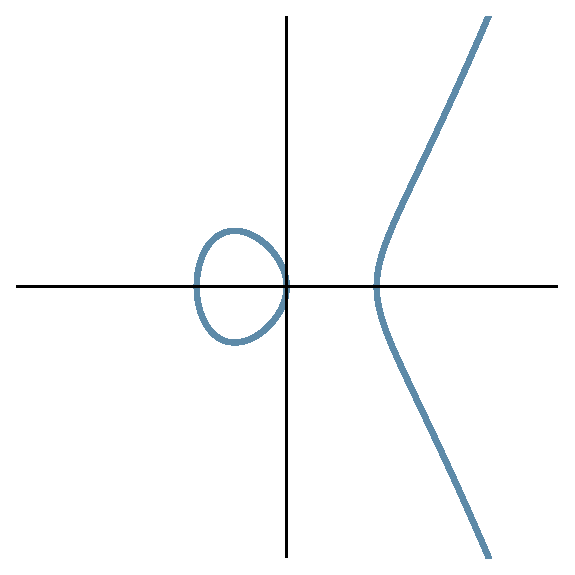
\includegraphics[width=\textwidth]{images/ec2.eps}
	\caption*{(a) $y^2=x(x^2+1)$}
	\end{subfigure}
	%
	\begin{subfigure}{0.35\textwidth}
	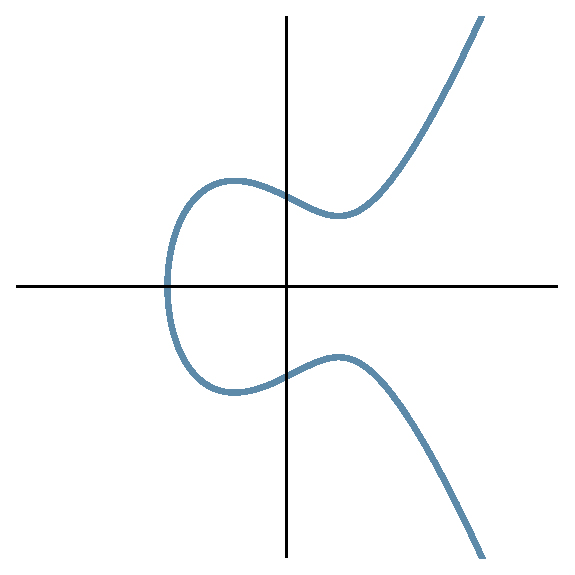
\includegraphics[width=\textwidth]{images/ec1.eps}
	\caption*{(b) $y^2=x^3-x+1$}
	\end{subfigure}
	\caption{An elliptic curve $y^2= x^3 + Ax + B$ with 3 real roots, (a), and 1 real root, (b).\label{fig:ellipticex}}
	\end{figure}


	\begin{figure}[!ht]
	\centering
	\begin{subfigure}{0.35\textwidth}
	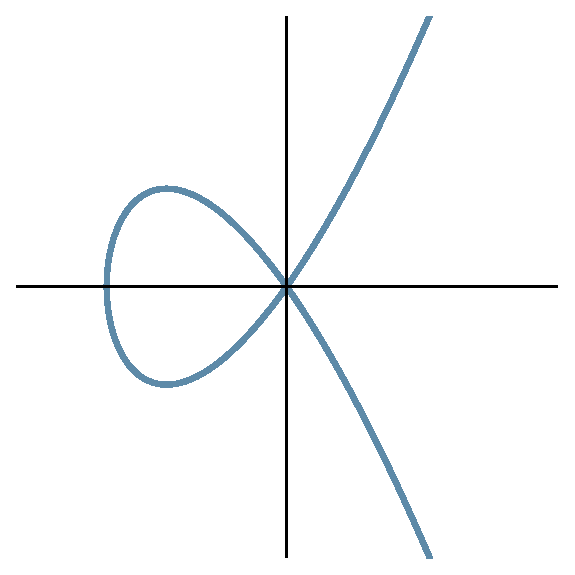
\includegraphics[width=\textwidth]{images/ec3.eps}
	\caption*{(a) $y^2=x^2(x+2)$}
	\end{subfigure}
	\begin{subfigure}{0.35\textwidth}
	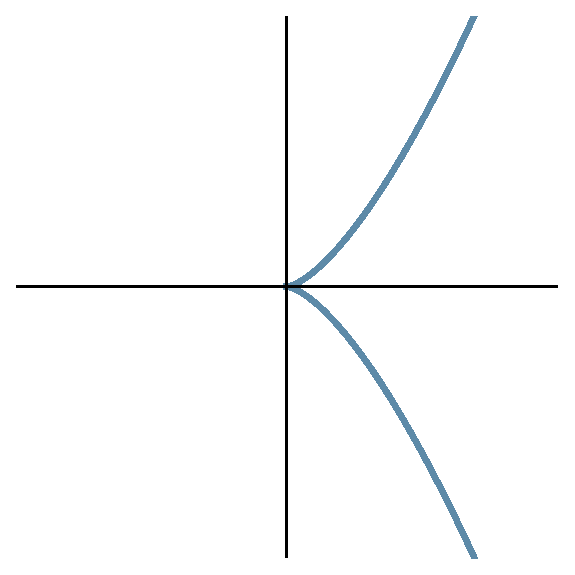
\includegraphics[width=\textwidth]{images/ec4.eps}
	\caption*{(b) $y^2= x^3$}
	\end{subfigure}
	\caption{An elliptic curve $y^2= x^3 + Ax + B$ with a node, (a), and a cusp, (b).\label{fig:singelliptic}}
	\end{figure}


We now define the addition law, which is given by the so-called Chord-Tangent Law, which we will also refer to as the geometric group law. Say $P$, $Q$ are two (distinct) $K$-rational points on an elliptic curve $E$, where for simplicity we say that $E$ has the form $y^2= x^3 + Ax + B$. Draw a line through $P$, $Q$. By B\'ezout's Theorem, this line will intersect the elliptic curve at another point, say $\widetilde{R}$. Reflect $\widetilde{R}$ across the $x$-axis (noting that in this form $(x,y) \in E$ if and only if $(x,-y) \in E$), and call this reflection point $R$. We then define $P +_E Q:= R$. If $P= Q$, then form the tangent line, and repeat this process, again defining $P +_E P:= R$. We take the identity under this `group law' (we have not proved this) to be $\cO$, the point at infinity. All of these constructions only involve ring operations in $K$, so that $R \in K \times K$, modulo a few minor technical difficulties, and the point $R$ is clearly on $E$. It is also immediately obvious from this construction that this `group law' is abelian. Moreover, inverses are clear: $P= (x,y)$ has inverse $-P= (x,-y)$. It only remains to show that the law is associative---which is a tour de force in case work and algebra too gratuitous to go into here. Indeed, in any case, one should prove the law is associative using Algebraic Geometry. A visualization of the Chord-Tangent Law is given in Figure~\ref{fig:chordtangent}, where the sum of the red and blue point is the yellow point. One can work out these operations explicitly, see \cite[III.2]{silvermanarithmetic} where one can also see how to handle the singular cases. 

	\begin{figure}[!ht]
	\centering
	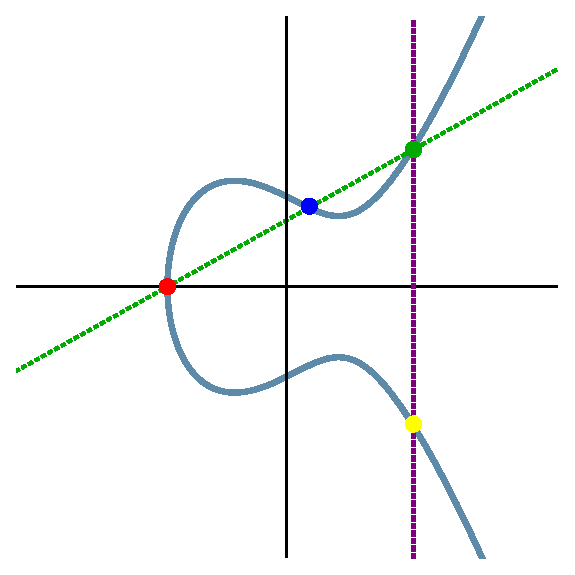
\includegraphics[width=0.47\textwidth]{images/ec_add.eps}
	\caption{The Chord-Tangent Law.\label{fig:chordtangent}}
	\end{figure}


All this discussion has (approximately) shown that definitions (ii) and (iii) for an elliptic curve are equivalent. But why is (i) equivalent to (ii)? Let $E$ be a smooth projective curve of genus 1 with a distinguished point $\cO$. There are functions $x,y \in K(E)$ such that the map $\phi: E \to \P^2$ given by $\phi= [x, y, 1]$ is an isomorphism to the definition of $E$ in (ii), see \cite[III.3, Prop.~3.1]{silvermanarithmetic}. This essentially follows from abstract nonsense involving examining the vector space $\cL(n\cO)$ for $n \in \N$ and applying the Riemann-Roch Theorem to then find an appropriate basis. Then if $P, Q \in E$, we have $(P) \sim (Q)$ if and only if $P= Q$. We then have the following proposition: 


\begin{prop}[{\cite[III.3, Prop.~3.4]{silvermanarithmetic}}]
Let $(E, \cO)$ be an elliptic curve. \leavevmode\vspace{-1em}
        \begin{enumerate}[(i)] \itemsep-1em
        \item For every degree-0 divisor $D \in \Div^0(E)$ there exists a unique point $P \in E$ satisfying $D \sim (P) - (\cO)$. Define $\sigma: \Div^0(E) \to E$ to be the map that sends $D$ to its associated $P$.
        \item The map $\sigma$ is surjective.
        \item Let $D_1, D_2 \in \Div^0(E)$. Then $\sigma(D_1)= \sigma(D_2)$ if and only if $D_1 \sim D_2$. Thus $\sigma$ induces a bijection of sets (which we also denote by $\sigma$), $\sigma: \Pic^0(E) \ma{\sim} E$. 
        \item The inverse to $\sigma$ is the map
        	\[
	\begin{aligned}
        	\kappa: E &\ma{\sim} \Pic^0(E), \\
	P &\mapsto \big(\text{divisor class of } (P) - (\cO) \big)
	\end{aligned}
        	\]
        \item If $E$ is given by a Weierstrass equation, then the ``geometric group law'' on $E$ and the ``algebraic group law'' induced from $\Pic^0(E)$ using $\sigma$ are the same. 
        \end{enumerate}
\end{prop}


\begin{cor}[{\cite[III.3, Cor.~3.5]{silvermanarithmetic}}]
Let $E$ be an elliptic curve and let $D= \sum n_p(P) \in \Div E$. Then $D$ is a principal divisor if and only if
	\[
	\sum_{P \in E} n_P= 0 \enskip\text{ and }\enskip \sum_{P \in E} [n_P]P= \cO.
	\]
(Note that the first sum is of integers, while the second is addition on $E$.)
\end{cor}


Using the fact that $E \cong \Pic^0(E)$, the associativity of the geometric group law then easily follows. This shows the equivalence of definitions (i) and (ii) for an elliptic curve. Note that of course the equivalence of (i) and (ii) in the definition of an elliptic curve requires choosing a specific affine chart. Choosing different affine charts will result in different forms for the elliptic curve, but these will all be isomorphic. We will be vague on the equivalence of (i) and (v) for an elliptic curve. Essentially if $\cC$ is a curve and $P \in \cC(K)$ is a $K$-rational point, we form the Jacobian variety of $\cC$ and the regular map $\phi: \cC \to J$ with $\phi(P)= 0$. `Extending linearly', the natural map from $\Div^0(\cC(K))$ to $J(K)$ is an isomorphism. 

Perhaps the most interesting equivalence for the definitions of an elliptic curve is between (iii) and (iv). We define a lattice, $\Lambda$, in $\C$ to be an additive subgroup of $\C$ generated by two $\R$-linearly independent complex periods $\omega_1, \omega_2 \in \C$, i.e. $\Lambda= \{ a\omega_1 + b\omega_2 \colon a,b \in \Z \}$, where $\omega_1:= a + ci$, $\omega_2:= b + di$ with $a,b,c,d \in \R$ are such that
	\[
	\det 
	\begin{pmatrix}
	a & b \\
	c & d 
	\end{pmatrix} \neq 0.
	\]
We say that two lattices $\Lambda, \Lambda'$ are homothetic if there is $u \in \C^\times$ such that $\Lambda'= u \Lambda$, i.e. one lattice can be scaled and rotated such that it then coincides with the other lattice. This implies that one can always choose $\omega= 1 \in \R$ by scaling. We call a fundamental domain (or the fundamental parallelogram) and its compactification, respectively, for a lattice to be
	\[
	\begin{aligned}
	\cF_\Lambda&= \{ a\omega_1 + b\omega_2 \colon  0 \leq a < 1, 0 \leq b < 1 \} \\
	\overline{\cF}_\Lambda&= \{ a\omega_1 + b\omega_2 \colon  0 \leq a < 1, 0 \leq b < 1 \}.
	\end{aligned}
	\]
Now as $\Lambda$ is an additive subgroup of $\C$, we can form the quotient $\C/\Lambda$. One can easily write down an isomorphism $\C/\Lambda \cong \cF_\Lambda$. You can also obtain this via ``gluing'' in $\overline{\cF}_\Lambda$, i.e. one can find an isomorphism $\C/\Lambda \cong \overline{\cF}_\Lambda/\sim$, where $\sim$ the identification of the opposite sides of the parallelogram $\overline{\cF}_\Lambda$. But of course, $\cF_\Lambda$ is isomorphic to $T:= S^1 \times S^1$, i.e. a complex torus. Routine verification checks that $\C/\Lambda$ inherits the topology induced from $\C$, and is homeomorphic to a torus via its identification with $\cF_\Lambda$. Moreover, $\C/\Lambda$ inherits the structure of a 1-dimensional complex manifold, so that $\C/\Lambda$ is a Riemann surface of genus 1, i.e. a complex torus. Two such tori, $\C/\Lambda$ and $\C/\Lambda'$, are isomorphic as Riemann surfaces if and only if $\Lambda, \Lambda'$ are homothetic.


Now we identify $\C/\Lambda$ with periodic meromorphic functions on $\C$. Define the Weierstrass $\wp$-function, $\wp(z)$, as 
	\[
	\wp(z):= \dfrac{1}{z^2} + \sum_{\omega \in \Lambda \setminus 0} \left( \dfrac{1}{(z - \omega)^2} - \dfrac{1}{\omega^2} \right). 
	\]
Lengthy but routine computations show that the sum on the right above converges absolutely, $\wp(z)$ is meromorphic and periodic, and that the only poles for $\wp(z)$ are double poles at every lattice point $\omega \in \Lambda$. Furthermore,
	\[
	\wp'(z)= -2 \sum_{\omega \in \Lambda} \dfrac{1}{(z- \omega)^3}
	\]
has poles only at the lattice points $\omega \in \Lambda$, and these are all triple poles. One then verifies that the function $\wp'(z)^2 - 4 \wp(z)^3 + g_2 \wp(z) + g_3$ has no poles, where
	\[
	\begin{aligned}
	G_{2k}&= \sum_{\omega \in \Lambda \setminus \{0\}} \dfrac{1}{\omega^{2k}} \\
	g_2&= 60 G_4 \\
	g_3&= 140 G_6.
	\end{aligned}
	\]
Furthermore, the numbers $g_2:= g_2(\Lambda)$ and $g_3:= g_3(\Lambda)$ depend only on the choice of lattice, and the sum $G_{2k}$ converges absolutely. It turns out, c.f. \cite[VI.3]{silvermanarithmetic}, that any doubly periodic function over $\C$ is a rational function in $\wp(z)$ and $\wp'(z)$, and that the extension $\C(\wp, \wp')/\C(\wp)$ is a quadratic extension. One then shows that $g_2^3 - 27g_3^2 \neq 0$. Then we define a mapping
	\[
	\begin{tikzcd}
	\C/\Lambda \arrow{r} & E(\C) \\ 
	z \rar[maps to] & \left( \wp(z), \wp'(z) \right),
	\end{tikzcd}
	\]
which is an (complex analytic) isomorphism of the complex Lie groups $\C/\Lambda$ and the elliptic curve $y^2= 4x^3 - g_2 x - g_3$,\footnote{Precisely, its homogenization, so that the map is rightfully $[\wp(z), \wp'(z), 1]$.} i.e. a map of complex Riemann surfaces that is also a group homomorphism. One checks that homothetic lattices $\Lambda$, $\Lambda'$ yield isomorphic elliptic curves. For the reverse direction, given an elliptic curve $y^2= 4x^3 - g_2 x - g_3$, we can take $\Lambda$ to be the lattice with periods $\omega_1, \omega_2$ given by
	\[
	\omega_1= \int_\alpha \dfrac{dx}{y} \quad\text{ and }\quad \omega_2= \int_\beta \dfrac{dx}{y},
	\]
where $\alpha, \beta$ are closed paths on $E(\C)$ that are a basis for $H_1(E, \Z)$. This is the so-called Uniformization Theorem, see \cite[IV.5, Thm.~5.1]{silvermanarithmetic}. The computation of $\omega_1, \omega_2$ is tedious and involves elliptic functions, choosing branch cuts, etc. However, if we can write $E$ in the form $y^2= (x - r_1)(x - r_2)(x - r_3)$ over $\C$ with $r_1, r_2, r_3 \in \R$ and $r_1 < r_2 < r_3$, then ignoring technical difficulties, we can write
	\[
	\begin{aligned}
	\omega_1&= \int_{r_1}^{r_2} \dfrac{dx}{\sqrt{(x - r_1)(x - r_2)(x - r_3)}} \\
	\omega_2&= \int_{r_2}^{r_3} \dfrac{dx}{\sqrt{(x - r_1)(x - r_2)(x - r_3)}}.
	\end{aligned}
	\]
This finally completes the equivalences of the definitions for an elliptic curve. 





% Mordell-Weil Theorem
\section{Mordell-Weil Theorem\label{sec:mordellweil}}

Now that we know an elliptic curve is a smooth projective curve of genus 1 (with a specified $K$-rational point $\cO$) with an addition structure, one might ask what this curve is as an abelian group. Poincar\'e conjectured in 1901 that the group $E(\Q)$ of rational points on an elliptic curve is a finitely generated abelian group \cite{poincare01}. This conjecture was proved by Mordell~\cite{mordell22} in 1922. Andr\'e Weil~\cite{weil29} then generalized Mordell's result in 1929, proving that the group of $K$-rational points on an abelian variety defined over a number field is a finitely generated abelian group.


\begin{thm}[Mordell-Weil, 1928] \label{thm:mordellweil}
Let $K$ be a number field, and let $A/K$ be an abelian variety. Then the group of $K$-rational points on $A$, denoted $A(K)$, is a finitely generated abelian group. In particular,
	\[
	A(K) \cong \Z^{r_K} \oplus A(K)_\tors,
	\]
where $r_K \geq 0$ is the rank of $A$ and $A(K)_\tors$ is the torsion subgroup.
\end{thm}


This was further generalized by N\'eron in \cite{neron52}. 


\begin{thm}[Mordell-Weil-N\'eron, 1952] \label{thm:bigmordellweil}
Let $K$ be a field that is finitely generated over its prime field, and let $A/K$ be an abelian variety. Then the group of $K$-rational points on $A$, denoted $A(K)$, is a finitely generated abelian group. In particular,
	\[
	A(K) \cong \Z^{r_K} \oplus A(K)_\tors,
	\]
where $r_K \geq 0$ is the rank and $A(K)_\tors$ is the torsion subgroup. 
\end{thm}


There exist further generalizations Lang-N\'eron~\cite{lang59}, see \cite{conradb} for further discussion. 


From the Mordell--Weil Theorem, it follows that $E(K) \cong \mathbb{Z}^{r_K} \oplus E(K)_\text{tors}$, where $r_K$ is the rank of the elliptic curve (depending on $K$) and $E(K)_\text{tors}$ is the torsion subgroup of $E$. Though vastly studied, there are very few concrete results on the ranks of elliptic curves $E/K$. Even in the case of $K= \Q$, it is not known what ranks are possible, or even if the ranks are unbounded, i.e. do there exist elliptic curves $E/\Q$ of arbitrary large rank. The current rank record is 29, due to Elikes. Table~\ref{tab:rankbound} summarizing rank records can be found in the database \cite{rankbound}.


	\begin{table}[!ht]
	\centering
	\caption{Rank records throughout history\label{tab:rankbound}}
	\begin{tabular}{lll} \hline
	Rank & Year & Due To \\ \hline
	3 & 1938 & Billing \\ 
	4 & 1945 &  Wiman \\ 
	6 & 1974 & Penney/Pomerance \\ 
	7 & 1975 & Penney/Pomerance \\
	8 & 1977 & Grunewald/Zimmert \\ 
	9 & 1977 & Brumer/Kramer \\
	12 & 1982 & Mestre \\ 
	14 & 1986 & Mestre \\
	15 & 1992 &  Mestre \\  
	17 & 1992 & Nagao \\
	19 & 1992 & Fermigier \\ 
	20 & 1993 & Nagao \\
	21 & 1994 & Nagao/Kouya \\ 
	22 & 1997 & Fermigier \\
	23 & 1998 & Martin/McMillen \\ 
	24 & 2000 & Martin/McMillen \\
	28 & 2006 & Elkies 
	\end{tabular}
	\end{table}


	\begin{figure}[!ht]
	\centering
	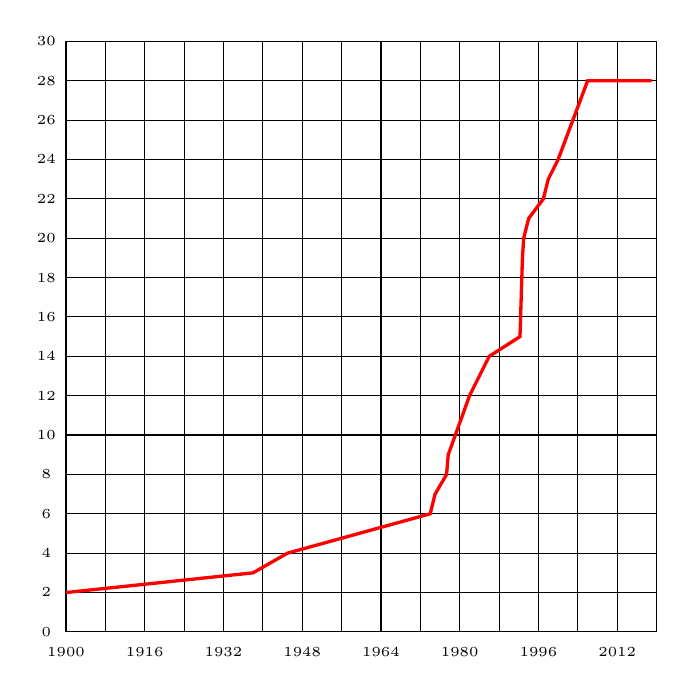
\begin{tikzpicture}[scale=0.50]%[scale=0.50, every node/.style={scale=0.1}]
	\foreach \k in {0,...,15}
		{
		\draw (\k,0) -- (\k,15);
		}
	\foreach \k in {0,...,15}
		{
		\draw (0,\k) -- (15,\k);
		}
	\node at (0,-0.5) {\tiny 1900};
	\node at (2,-0.5) {\tiny 1916};
	\node at (4,-0.5) {\tiny 1932};
	\node at (6,-0.5) {\tiny 1948};
	\node at (8,-0.5) {\tiny 1964};
	\node at (10,-0.5) {\tiny 1980};
	\node at (12,-0.5) {\tiny 1996};
	\node at (14,-0.5) {\tiny 2012};
	
	\node at (-0.5,0) {\tiny 0};
	\node at (-0.5,1) {\tiny 2};
	\node at (-0.5,2) {\tiny 4};
	\node at (-0.5,3) {\tiny 6};
	\node at (-0.5,4) {\tiny 8};
	\node at (-0.5,5) {\tiny 10};
	\node at (-0.5,6) {\tiny 12};
	\node at (-0.5,7) {\tiny 14};
	\node at (-0.5,8) {\tiny 16};
	\node at (-0.5,9) {\tiny 18};
	\node at (-0.5,10) {\tiny 20};
	\node at (-0.5,11) {\tiny 22};
	\node at (-0.5,12) {\tiny 24};
	\node at (-0.5,13) {\tiny 26};
	\node at (-0.5,14) {\tiny 28};
	\node at (-0.5,15) {\tiny 30};
	
	\draw[very thick,red] plot[samples=500] coordinates {
	(0,1)
	(4.75,1.5)
	(5.625,2)
	(9.25,3)
	(9.375,3.5)
	(9.6667,4)
	(9.7083,4.5)
	(10.25,6)
	(10.75,7)
	(11.5313,7.5)
	(11.5625,8.5)
	(11.5938,9.5)
	(11.625,10)
	(11.75,10.5)
	(12.125,11)
	(12.25,11.5)
	(12.5,12)
	(13.25,14)
	(14.875,14)
	};
	\end{tikzpicture}
	\caption{Rank records over time.}
	\end{figure}


The greatest successes in the direction of studying ranks has come from examining how the ranks can grow in towers of number fields, where one employs techniques from Iwasawa Theory. However, this is far beyond our scope. There are suggestions that the ranks of elliptic curves may be bounded. In a recent paper of Machett Wood, Park, Poonen, and Voight \cite{parkpoonenvoightwood19}, by modeling Shafarevich-Tate groups using certain alternating matrices of specified ranks, they predict that there only finitely many elliptic curves (up to isomorphism) with rank greater than 21. However, data analyzed by \lozrob{} in \cite{lozanorobledo21} using statistical modeling suggests that there may still be infinite families with large rank. In any case, the rank of an elliptic curve is ``typically'' small. Specifically, that ``most'' elliptic curves either have rank 0 or 1. This is commonly referred to as the minimalist conjecture. We will only comment on this briefly. To prove the Mordell-Weil Theorem (there is essentially only one proof, they all boil down to the same idea), one must prove that $E(\Q)/nE(\Q)$ is finite for some $n \geq 2$---typically $n= 2$. This is a vast generalization of the descent technique of Fermat. Let $\Q_p$ be the $p$-adic numbers, where we allow $p= \infty$, i.e. $\Q_\infty= \R$, and fix an algebraic closure $\ov{\Q}$ of $\Q$. Denote by $H^1(\Q, E)$ the profinite cohomology group $H^1(\Gal(\ov{\Q}/\Q), E(\ov{\Q}))$. We take Galois cohomology of the exact sequence
	\[
	0 \ma{} E[n] \ma{} E \ma{[n]} E \ma{} 0
	\]
over $\Q$ and $\Q_p$ for each prime $p$, which gives a long exact sequence (the Kummer sequence), from which we can obtain the following commutative diagram
	\[
	\begin{tikzcd}
	0 \arrow{r} & E(\Q)/nE(\Q) \arrow{r} \arrow{d} & H^1(\Q, E[n]) \arrow{d}{\iota_1} \arrow{r} & H^1(\Q,E)[n] \arrow{d} \arrow{r} & 0 \\
	0 \arrow{r} & \prod_{p \leq \infty} E(\Q_p)/nE(\Q_p) \arrow{r}{\iota_2} & \prod_{p \leq \infty} H^1(\Q_p, E[n]) \arrow{r} & \prod_{p \leq \infty} H^1(\Q_p,E)[n] \arrow{r} & 0 
	\end{tikzcd}
	\]
Because the group $H^1(\Q, E[n])$ is cumbersome to work with, we choose to work locally over $\Q_p$. We then define the $n$-Selmer group
	\[
	\sel_n(E):= \{ x \in H^1(\Q, E[n]) \colon \im \iota_1 \in \im \iota_2 \}.
	\]
Then $\sel_n E \subseteq H^1(\Q, E[n])$ bounds $E(\Q)/nE(\Q)$. The group $\sel_n E$ is finite and computable---though this is highly non-trivial. We then define the Shafarevich-Tate group
	\[
	\sha_E:= \ker \left( H^1(\Q, E) \ma{} \prod_{p \leq \infty} H^1(\Q_p, E) \right),
	\]
which then gives an exact sequence
	\[
	0 \ma{} E(\Q)/nE(\Q) \ma{} \sel_n E \ma{} \sha[n] \ma{} 0.
	\]
It is not known whether $\sha_E$ is finite---although that is the conjecture. Measuring the ``average'' size of Selmer groups, Bhargava and Shankar \cite{bhargavashankar15} prove that the ``average'' rank of elliptic curves is at most 7/6 in the sense that 
	\[
	\lim_{X \to \infty} \dfrac{\sum_{\height E < X} \rank E}{\sum_{\height E < X} 1} \leq \dfrac{7}{6}, 
	\]
which we shall not make any more precise. Again, this limit is conjectured to be $\frac{1}{2}$, the so-called ``50-50 conjecture.'' Goldfeld has also conjectured that the probability
	\[
	\lim_{D \to \infty} \dfrac{\# \{ E^{(d)} \colon d \leq D, \rank E^{(d)} \geq 1 \}}{\#\{ E^{(d)} \colon d \leq D \}}= \dfrac{1}{2}. 
	\]
This is typically referred to as Goldfeld's conjecture. We will not make this any more precise. For more on both of these problems, see \cite{bektemirovmazursteinwatkins07} and \cite{poonen15}. Note that Shafarevich and Tate \cite{shatate67} showed that the rank of elliptic curves over function fields is unbounded. There is a conjectural formula to compute the rank of an elliptic curve, namely the \$1~million prize problem of Birch and Swinnerton-Dyer:
	\[
	\lim_{s \to 1} \dfrac{L(E,s)}{(s-1)^{r_E}} \stackrel{?}{=} \dfrac{\Omega_E \, \Reg(E) \, \#\sha(E/\Q) \, \prod_p c_p}{\#E(\Q)_{tors}^2},
	\]
where $L(E,s)$ is the $L$-function associated to $E$, $r_E$ is the rank of $E$, $\Omega_E= \int_{E(\R)} \left| \frac{dx}{y} \right|$, $\Reg(E)$ is the regulator of $E$, and $c_p$ is Tamagawa number, i.e. cardinality of $E(\Q_p)/E_0(\Q_p)$ where $E_0(\Q_p)$ is the set of points in $E(\Q_p)$ whose mod $p$ reductions is nonsingular in $E(\F_p)$. 


While the ranks are quite intractable, the torsion subgroup is much better understood. Treating an elliptic curve $E$ as $\C/\Lambda$, we can easily see that the subgroup of points of order $n$,\footnote{By abuse of language, we will say points of order $n$ to mean points $P \in E$ such that $nP= \cO$.} denoted $E[n]$, is isomorphic to $\Z/n\Z \oplus \Z/n\Z$, this is demonstrated for $n= 4$ in Figure~\ref{fig:e4} \cite{periodparallelogram}. 

	\begin{figure}[h]
	\centering
	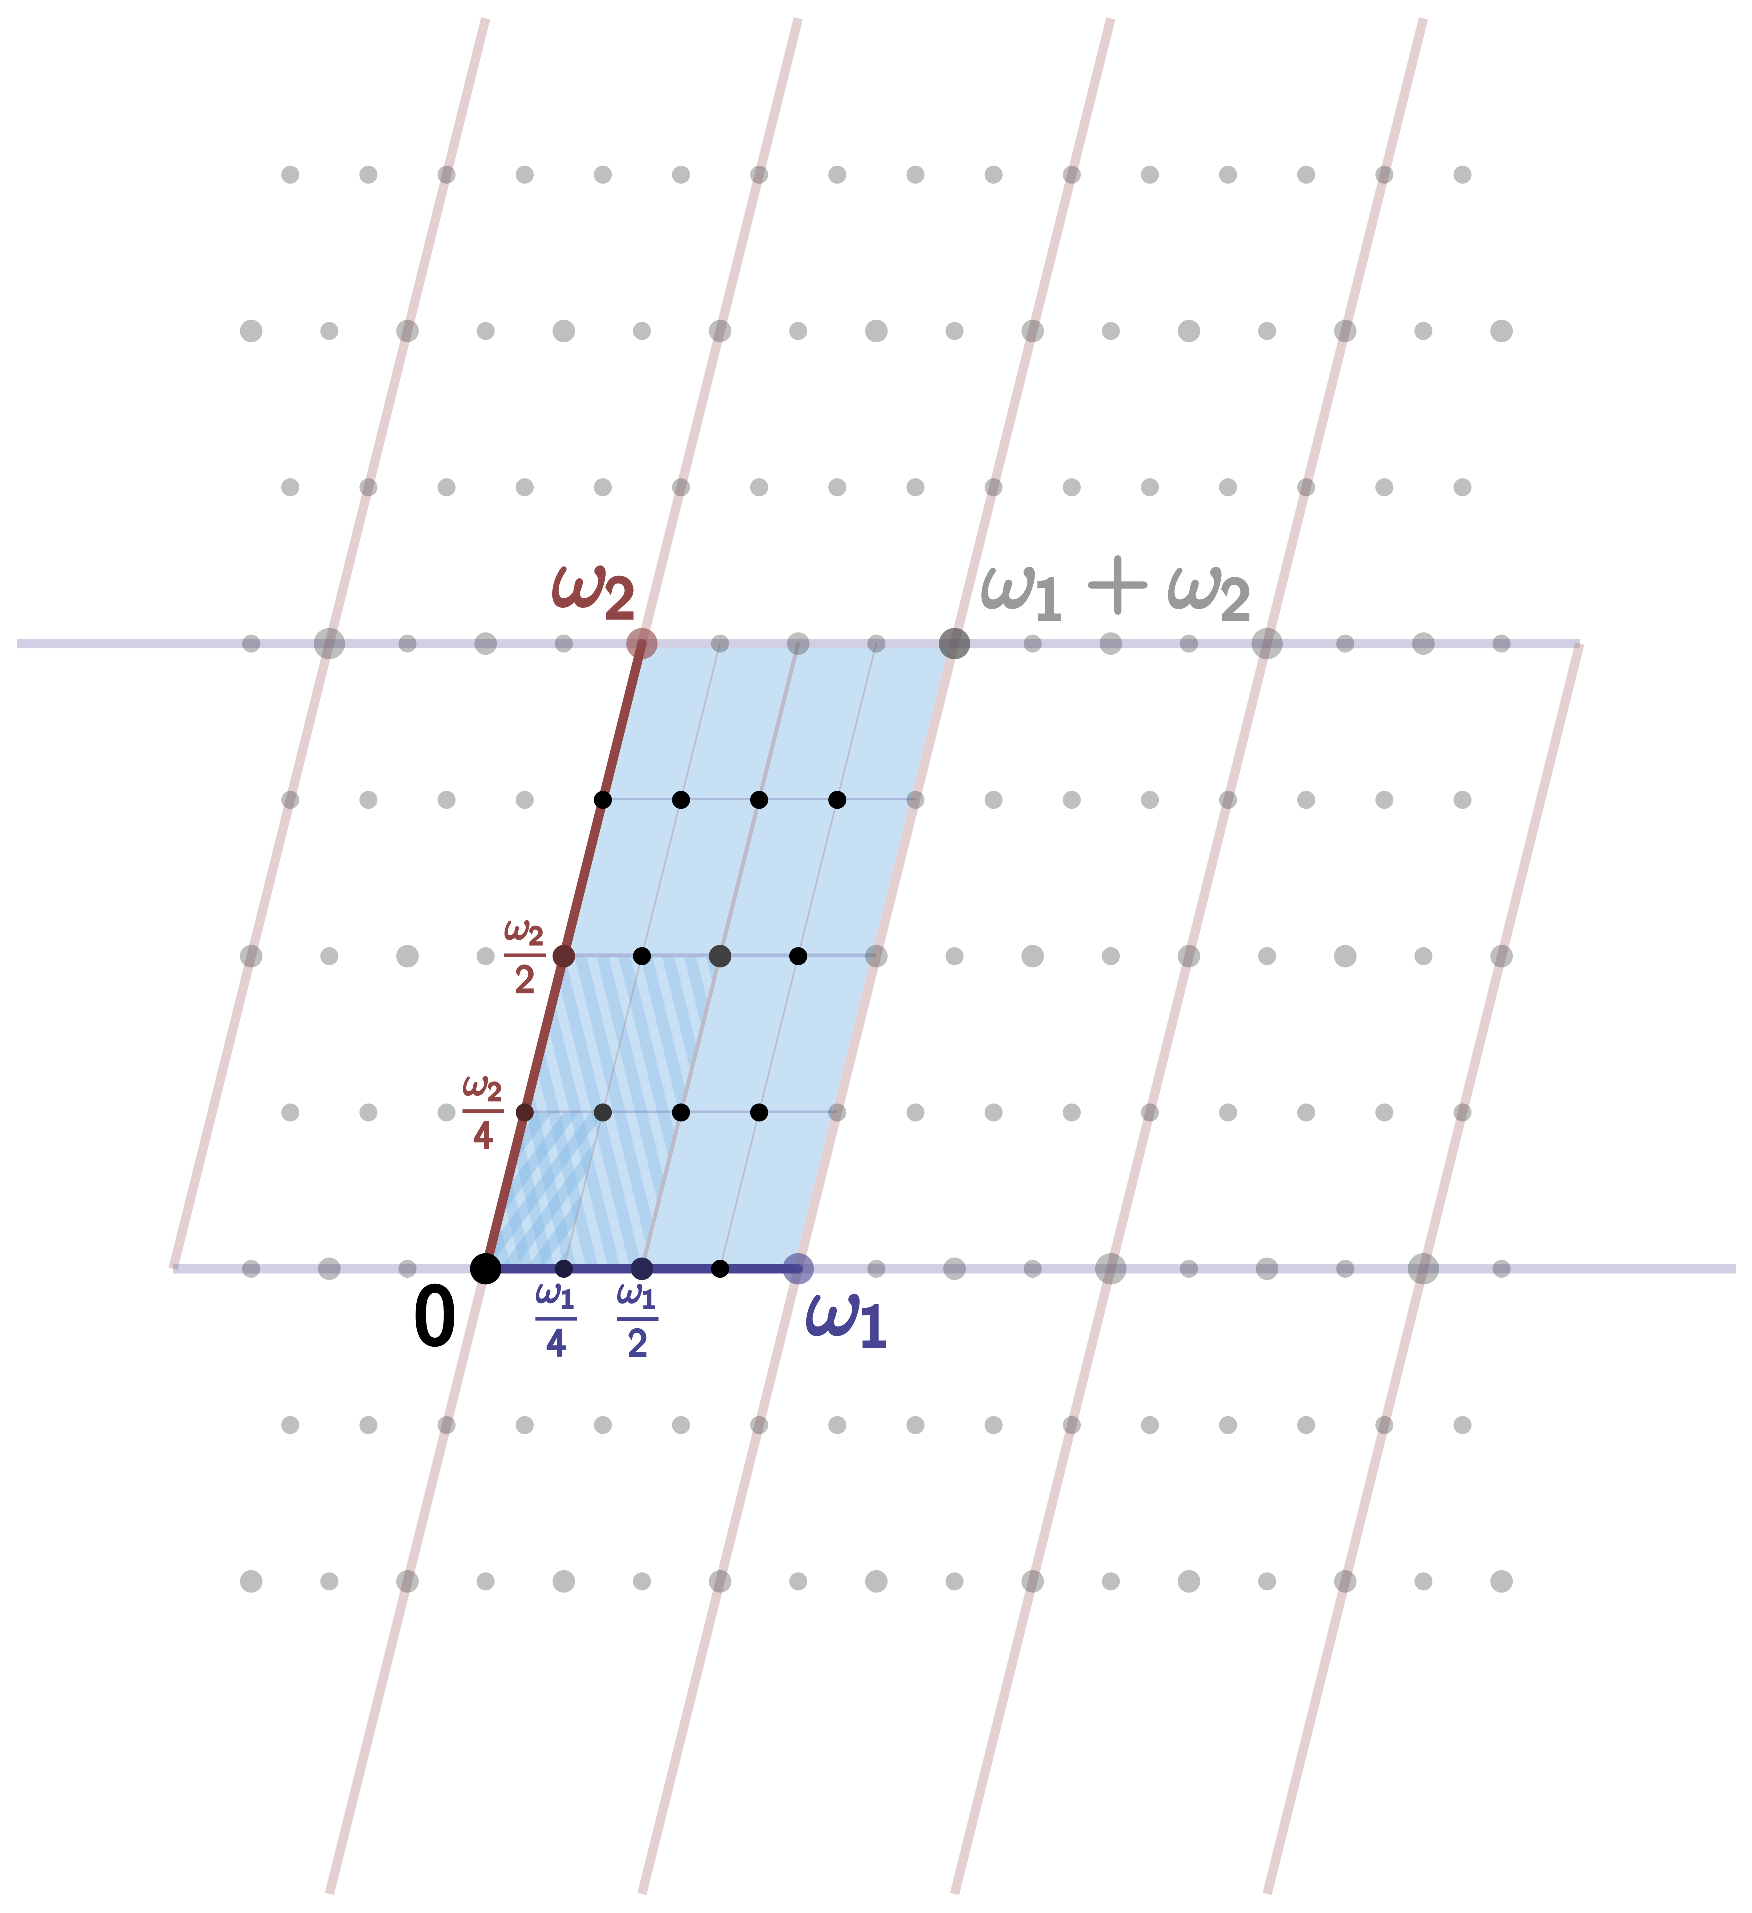
\includegraphics[width=0.40\textwidth]{images/lattice.eps}
	\caption{The subgroup $E[4]$ via the period parallelogram.\label{fig:e4}}
	\end{figure}
If instead we restrict to the points of order $n$ defined over a field $K$ (rather than over $\C$), it is well-known (see \cite{silvermanarithmetic}) that $E(K)_\text{tors} \cong \mathbb{Z}/n\mathbb{Z} \oplus \mathbb{Z}/nm\mathbb{Z}$, where $n,m \geq 1$ are positive integers. Generally, if $A/K$ is an abelian variety with genus $g$, $A(K)_\tors$ is a $\Z/n\Z$-module of rank $2g$. Furthermore, fixing a genus $g$, given a possible torsion subgroup (that is, one compatible with the genus), there is an abelian variety over some field with that specified torsion subgroup. 


Finally, we mention in passing two amazing theorems concerning the structure of integral points on elliptic curves.


\begin{thm}[{Siegel,\cite[IX.3, Thm.~3.1]{silvermanarithmetic}}] \label{thm:siegel}
Let $E/\Q$ be an elliptic curve. Then the set of integral points on $E$ is finite. 
\end{thm}


There are ineffective bounds on the size of these integral points due to Baker \cite{baker90} in terms of $A, B$: if $(x,y)$ is an integral point on $E: y^2= x^3 + Ax + B$, the
	\[
	\max\{|x|, |y| \} \leq \exp\left(\left(10^6 \cdot \max\{ |A|, |B|\} \right)^{10^6} \right).
	\]


\begin{thm}[{Nagell-Lutz, \cite{nagell35,lutz37}}]
Let $E/\Q$ be an elliptic curve with equation $y^2= x^3 + Ax + B$, $A, B \in \Z$. If $P \in E(\Q)$ is a nonzero torsion point, then $x(P)$, $y(P) \in \Z$ and either $y= 0$, i.e. $[2]P= \cO$, or $y(P)^2$ divides $4A^3 + 27B^2$. 
\end{thm}





% Isogenies 
\section{Isogenies\label{sec:isog}}

Now that we have defined elliptic curves, we want to define maps between them. These will be isogenies. Note that one makes similar definitions in the case of abelian varieties $A/K$. 


\begin{dfn}
Let $E_1$ and $E_2$ be elliptic curves. An isogeny from $E_1$ to $E_2$ is a morphism $\phi: E_1 \to E_2$ with $\phi(\cO)= \cO$. Two elliptic curves $E_1$ and $E_2$ are isogenous if there is an isogeny from $E_1$ to $E_2$ with $\phi(E_1) \neq \{ \cO \}$. 
\end{dfn}


From routine Algebraic Geometry, a map of projective curves is either surjective or constant, see \cite[II.2.3]{silvermanarithmetic}. Hence for an isogeny of elliptic curves, we either have $\phi(E_1)= \{ \cO \}$ or $\phi(E_1)= E_2$. But the only isogeny with $\phi(E_1)= \{ \cO \}$ is the zero isogeny given by $[0](P)= \cO$ for all $P \in E_1$. Though it is not immediately obvious, isogenies form an equivalence relation (this follows from the existence of the dual isogeny). We have a map of function fields, $\phi^*: \ov{K}(E_2) \to \ov{K}(E_1)$, which by our preceding comments must be an injection.  


The degree of an isogeny $\phi$, which we will denote by $\deg \phi$, is the degree of the finite extension $\ov{K}(E_1)/\phi^*\ov{K}(E_2)$. We define similarly the separable and inseparable degrees for $\phi$, denoted respectively by $\deg_s \phi$ and $\deg_i \phi$, respectively. We also refer to the map $\phi$ as being separable, inseparable, or purely inseparable according to the corresponding property of the field extension. By convention, we set $\deg [0]= 0$ so that $\deg(\psi \circ \phi)= \deg \psi \deg \phi$ for maps $E_1 \ma{\phi} E_2 \ma{\psi} E_3$. Because elliptic curves are abelian groups, one can then form $\Hom(E_1, E_2)$ to be the group of isogenies in the usual way. Similarly, one defines $\End E:= \Hom(E, E)$ in the usual way, where addition is addition on the elliptic curve and multiplication is given by function composition. Then $\Aut E$ is the set of invertible endomorphisms. Of course, if $E$ is defined over some field $K$, one may restrict $\Hom(E_1, E_2)$, $\End E$, $\Aut E$ to just those maps defined over $K$. 


Observe that the definition of an isogeny mentions nothing about the fact that the morphisms respect the group law on the elliptic curve. However, it is the case that every isogeny is a homomorphism of elliptic curves (the reverse is also true). 


\begin{thm}[{\cite[III.4.8]{silvermanarithmetic}}]
Let $\phi: E_1 \to E_2$ be an isogeny. Then $\phi(P + Q)= \phi(P) + \phi(Q)$ for all $P, Q \in E_1$.
\end{thm}


\begin{cor}[{\cite[III.4.9]{silvermanarithmetic}}]
Let $\phi: E_1 \to E_2$ be a nonzero isogeny. Then $\ker \phi= \phi^{-1}(\cO)$ is a finite group.
\end{cor}


For an isogeny $\phi: E_1 \to E_2$ with $\#\ker \phi= n$, we say that $E_1$ has a $n$-isogeny. If the map $\phi$ is defined over a field $K$, we say that $E_1$ has a $K$-rational $n$-isogeny. Finally, if $\ker \phi$ is cyclic, we say that $E$ has a cyclic isogeny. Typically, throughout this work, whenever we refer to an isogeny, we will mean a rational cyclic isogeny. 


\begin{ex}
For each $m \in \Z$ we define the multiplication-by-$n$ isogeny $[n]: E \to E$ in the natural way, i.e. $[n](P)$ is the $n$-fold sum of $P$ on $E$. Moreover, this map is an isogeny as it sends $\cO$ to $\cO$. 
\end{ex}


\begin{prop}[{\cite[III.4.2]{silvermanarithmetic}}]
Let $E_1/K$ and $E_2/K$ be elliptic curves, and let $n \in \Z$ with $n \neq 0$. Then the multiplication-by-$n$ map $[n]: E \to E$ is nonconstant. Furthermore, the group of isogenies $\Hom(E_1, E_2)$ is a torsion-free $\Z$-module and $\End E$ is a ring of characteristic 0 with no zero divisors (not necessarily commutative). 
\end{prop}


Typically, $\End E \cong \Z$ and is entirely composed of the multiplication-by-$n$ maps, i.e. the map $\Z \to \End E$ given by $n \mapsto [n]$ is an isomorphism. Over fields of characteristic 0, this map is always injective so that we can view $\Z \subseteq \End E$.\footnote{Over finite fields, $\End E$ is always strictly larger than $\Z$.} However, there are elliptic curves where this inclusion is strict. 


\begin{ex}[{\cite[III.4.4]{silvermanarithmetic}}]
Let $K$ be a field with $\ch K \neq 2$, and let $i \in \ov{K}$ be a primitive fourth root of unity, i.e. $i^2= -1$. Consider the elliptic curve $E/K$ given by $y^2= x^3 - x$. Observe that we have a map $[i]: E \to E$ given by $(x,y) \mapsto (-x,iy)$. Note that $[i]$ is defined over $K$ if and only if $i \in K$, but that $E$ is certainly defined over $K$. Furthermore, observe that
	\[
	[i] \circ [i](x,y)= [i](-x,iy)= (x,-y)= -(x,y),
	\]
so that $[i] \circ [i]= [-1]$. We then have a ring homomorphism $\Z[i] \to \End E$ given by $m + ni \mapsto [m] + [n] \circ [i]$. Assuming $\ch K= 0$, this map is an isomorphism, i.e. $\Z[i] \cong \End E$. Then $\Aut E \cong \Z[i]^*= \{ \pm 1, \pm i \}$ is a cyclic group of order 4. Elliptic curves with $\End E \supsetneq E$ are said to have CM, or are simply called CM elliptic curves. It is no coincidence that in this example that the endomorphism ring was the ring of integers in an imaginary quadratic field. 
\end{ex}


With the multiplication-by-$n$ map defined, we can then properly define the $n$-torsion subgroup of $E$. 


\begin{dfn}[$n$-torsion subgroup]
Let $E$ be an elliptic curve, and let $n \in \Z$ with $n \geq 1$. The $n$-torsion subgroup of $E$, denoted by $E[n]$, is the set of points of $E$ of order $n$, $E[m]= \{ P \in E \colon [n]P= \cO \}$. The torsion subgroup of $E$, denoted by $E_\tors$ is the set of points of finite order $E_\tors= \bigcup_{m=1}^\infty E[m]$. If $E$ is defined over $K$, then $E_\tors(K)$ denoted the point of finite order in $E(K)$. 
\end{dfn}


It is worth noting that one can construct isogenies from finite subgroups of $E$. 


\begin{prop}[{\cite[III.4.12]{silvermanarithmetic}}] \label{prop:velulem}
Let $E$ be an elliptic curve and let $\Phi$ be a finite subgroup of $E$. There are a unique elliptic curve $E'$ and a separable isogeny $\phi: E \to E'$ satisfying $\ker \phi= \Phi$.
\end{prop}


If $E$ is defined over $K$ and $\Phi$ is $G_{\ov{K}/K}$-invariant, i.e. $T^\sigma \in \Phi$ for all $\sigma \in G_{\ov{K}/K}$, then the curve $E'$ and isogeny $\phi$ can be defined over $K$. There are descriptions on how to construct equations for $E'$ and the isogeny $\phi: E \to E'$, c.f. \cite{velu71}. 


Finally, although we will not make much use of it, for every nonconstant isogeny of elliptic curves $\phi: E_1 \to E_2$ of degree $n$, there is an isogeny, denoted $\widehat{\phi}: E_2 \to E_1$ with $\widehat{\phi} \circ \phi= [n]$. If $\phi= [0]$, we take $\widehat{\phi}= [0]$. 


\begin{thm}[{\cite[III.6.2]{silvermanarithmetic}}]
Let $\phi: E_1 \to E_2$ be an isogeny of elliptic curves. Then \leavevmode\vspace{-3em}
        \begin{enumerate}[(a)] \itemsep-1em
        \item Let $m= \deg \phi$. Then $\hat{\phi} \circ \phi= [m]$ on $E_1$ and $\phi \circ \hat{\phi}= [m]$ on $E_2$
        \item Let $\lambda: E_2 \to E_3$ be another isogeny. Then $\hat{\lambda \circ \phi}= \hat{\phi} \circ \hat{\lambda}$.
        \item Let $\psi: E_1 \to E_2$ be another isogeny. Then $\hat{\phi + \psi}= \hat{\phi} + \hat{\psi}$.
        \item For all $m \in \Z$, $\hat{[m]}= [m] \text{ and } \deg [m]= m^2$.
        \item $\deg \hat{\phi}= \deg \phi$
        \item $\hat{\hat{\phi}}= \phi$. 
        \end{enumerate}
\end{thm}


For more on dual isogenies, see \cite[III.6]{silvermanarithmetic}. 





% Weil Pairing
\section{Weil Pairing\label{sec:weilpair}}

Let $E/K$ be an elliptic curve, where $K$ is a field of characteristic $p$. Fix an integer $n \geq 2$, where if $p= \ch K > 0$  we assume that $\gcd(n,p)= 1$. We know that the group of $n$-torsion points is $E[n] \cong \Z/n\Z \oplus \Z/n\Z$. Therefore, $E[n]$ is a free $\Z/n\Z$-module of rank two. We define an alternating, nondegenerate multilinear map on $E[n]$. Fix a $\Z/n\Z$-basis for $E[n]$, say $\{ P, Q \}$. We then have a determinant map:
	\[
	\begin{aligned}
	\det: E[n] \times E[n] &\to \Z/n\Z \\
	\det(aP + bQ,& cP + dQ):= ad - bc.
	\end{aligned}
	\]
Of course, the values of this map depend on the choice of basis. However, selecting a different basis simply scales all of the values of $\det: E[n] \times E[n] \to \Z/n\Z$ by an element of $(\Z/n\Z)^\times$. Note also that this map is not Galois invariant: if $P, Q \in E[n]$ and $\sigma \in G_{\ov{K}/K}$, then $\det(P^\sigma, Q^\sigma)$ need not be the same as $\det(P,Q)^\sigma$. It would be advantageous to have a `determinant' map which is Galois invariant. For this, we need the pairing to take values in the $n$th roots of unity. To create such a pairing, we make use of the fact that if $E$ is an elliptic curve and $D= \sum n_P(\cO) \in \Div(E)$, then $D$ is a principal divisor if and only if $\sum_{P \in E} n_P= 0$ and $\sum_{P \in E} [n_P]P= \cO$. 


Suppose that $T \in E[n]$. There is then a function $f \in \ov{K}(E)$ with $\div f= n(T) - n(\cO)$. Let $T' \in E$ be a point with $[n]T'= T$. Similarly, we have a function $g \in \ov{K}(E)$ satisfying
	\[
	\div g = [m]^*(T) - [m]^*(\cO) = \sum_{R \in E[n]} \big( (T' + R) - (R) \big).
	\]
It is routine to check that $f \circ [n]$ and $g^m$ have the same divisor. Scaling $f$, we can assume that $f \circ [n]= g^n$. 


Now suppose that $S \in E[n]$ is an $n$-torsion point (not necessarily distinct from $T$). For $X \in E$, 
	\[
	g(X + S)^m= f([m]X + [m] S)= f([m]X)= g(X)^m.
	\]
Then the function $e_m(X):= g(X + S)/g(X)$ has finite image. But then for all $X$, $e(X)$ is an $n$th root of unity. The map of curves, $E \to \bP$ given by $e_m(X)$ then cannot be surjective. But maps of curves are constant or surjective. Therefore, $F(X)$ is constant. 


We then define a pairing $e_n \colon E[n] \times E[n] \to \mu_n$ by defining $e_n(S,T)= \dfrac{g(X + S)}{g(X)}$, where $X \in E$ is any point such that $g(X + S)$ and $g(X)$ are well-defined and nonzero. While the function $g$ is defined only up to multiplication by some $\alpha \in \ov{K}^\times$, the value of $e_n(S,T)$ is independent of the choice of $\alpha$. 


\begin{dfn}[Weil Pairing]
We define the map $e_n(S,T)$ described above is called the Weil ($e_n$-)pairing. 
\end{dfn}


There is alternative construction of the Weil pairing. Choose $X, Y \in E$ and $f_S, f_T \in \ov{K}(E)$ with $\div f_S= m(X + S) - m(X)$ and $\div f_T= M(Y + T) - m(Y)$. Then one can define the pairing 
	\[
	e_m(S,T) = \dfrac{f_S(Y + T)}{f_S(Y)} \bigg\slash \dfrac{f_T(X + S)}{f_T(X)},
	\]
though one need check that this map is well defined and is the same as the Weil pairing defined above. 


\begin{prop}[{\cite[III.8.1]{silvermanarithmetic}}]
The Weil $e_n$-pairing has the following properties: \leavevmode\vspace{-1em}
	\begin{enumerate}[(a)] \itemsep-1em
	\item It is bilinear
		\[
		\begin{aligned}
		e_n(S_1 + S_2, T)&= e_n(S_1,T) e_n(S_2,T) \\
		e_n(S, T_1 + T_2)&= e_n(S,T_1) e_n(S,T_2) 
		\end{aligned}
		\]
	\item It is alternating: $e_n(T,T)= 1$.
	\item It is nondegenerate: if $e_n(S,T)= 1$ for all $S \in E[n]$, then $T= \cO$.
	\item It is Galois invariant: $e_n(S,T)^\sigma= e_n(S^\sigma,T^\sigma)$ for all $\sigma \in G_{\ov{K}/K}$.
	\item It is compatible: $e_{nn'}(S,T)= e_n([n']S, T)$ for all $S \in E[nn']$ and $T \in E[n]$. 
	\end{enumerate}
\end{prop}


The existence of the Weil pairing forces the following useful fact about fields over which full $n$-torsion can be defined.


\begin{cor}[{\cite[III.8.1.1]{silvermanarithmetic}}] \label{cor:weilpairing}
There exist points $S, T \in E[n]$ such that $e_n(S,T)$ is a primitive $m$th root of unity. In particular, if $E[n] \subset E(K)$, then $\mu_n \subset K^\times$. 
\end{cor}

\begin{proof}
We give the proof in \cite{silvermanarithmetic}. The image of $e_n(S,T)$ as $S$ and $T$ range over $E[n]$ is a subgroup of $\mu_n$, say equal to $\mu_d$. It follows that
	\[
	1= e_n(S,T)^d= e_n([d]S, T) \text{ for all } S,T \in E[n].
	\]
The nondegeneracy of the $e_n$-pairing implies that $[d]S= \cO$, and since $S$ is arbitrary, it follows from \cite[III.6.4]{silvermanarithmetic} that $d= n$. Finally, if $E[n] \subset E(K)$, then the Galois invariance of the $e_n$-pairing implies that $e_n(S,T) \in K^*$ for all $S,T \in E[n]$. Hence, $\mu_n \subset K^*$. 
\end{proof} 


If $\phi: E_1 \to E$ is an isogeny, and $\hat{\phi}$ its corresponding dual isogeny, then $\phi, \hat{\phi}$ are dual (or adjoint) with respect to the Weil pairing, see \cite[III.8.2]{silvermanarithmetic}


\begin{prop}
Let $\phi: E_1 \to E_2$ be an isogeny of elliptic curves. Then for all $m$-torsion points $S \in E_1[m]$ and $T \in E_2[m]$, $e_m(S, \hat{\phi}(T))= e_m(\phi(S),T)$.
\end{prop}


For a prime $\ell$, one can combine the various $e_{\ell^n}$ pairings compatibly to define a $\ell$-adic Weil pairing on the $\ell$-adic Tate module, $T_\ell(E):= \plim E[\ell^n]$, where the limit is taken over the natural maps $E[\ell^{n+1}] \ma{[\ell]} E[\ell^n]$, which we will not go into here. 


But this turns out to be extremely useful. The resulting Weil pairing action on the $\ell$-adic Tate module $T_\ell$ gives a determinant and trace map. Viewing the Tate module as a homology group, we can then compute the degrees of isogenies topologically by examining its action on $H_1(E, \Z_\ell)$. This gives a way of computing points on elliptic curves over finite fields. 


\begin{prop}[{\cite[III.8.6]{silvermanarithmetic}}]
Let $\phi \in \End E$ and $\phi_\ell: T_\ell(T) \to T_\ell(E)$ be the map that $\phi$ induces on the Tate module of $E$. Then 
	\[
	\det \phi_\ell= \deg \phi \text{ and } \tr(\phi_\ell)= 1 + \deg \phi - \deg(1 - \phi),
	\]
where $\phi_\ell$ comes from the representation $\End E \to \End T_\ell(E)$ given by $\phi \mapsto \phi_\ell$. In particular, $\det \phi_\ell$ and $\tr \phi_\ell$ are in $\Z$ and are independent of $\ell$. 
\end{prop}





% The Endomorphism and Automorphism Groups
\section{The Endomorphism and Automorphism Groups\label{sec:endaut}}

Let $E$ be an elliptic curve. It is well known that $\End E$ has characteristic 0, no zero divisors, and rank at most 4 when viewed as a $\Z$-module; moreover, $\End E$ has an anti-involution: $\phi \mapsto \hat{\phi}$, for $\phi \in \End E$ the product $\phi \,\hat{\phi}$ is a non-negative integer and further $\phi \,\hat{\phi}= 0$ if and only if $\phi= 0$, see \cite[\S III]{silvermanarithmetic}. Suppose that $\cK$ is a (not necessarily commutative) $\Q$-algebra that is also finitely generated over $\Q$. We call $\cR$ an order of $\cK$ if it is a subring of $\cK$ that is finitely generated as a $\Z$-module and satisfies $\cR \otimes \Q= \cK$. To give the possibilities for $\End E$, we will need the following definition: 


\begin{dfn}[(Definite) Quaternion Algebra]
A (definite) quaternion algebra is an algebra of the form $\cK= \Q + \Q \alpha + \Q \beta + \Q \alpha \beta$, whose multiplication satisfies $\alpha^2, \beta^2 \in \Q$, $\alpha^2 < 0$, $\beta^2 < 0$, and $\beta\alpha= -\alpha\beta$.
\end{dfn}


\begin{thm}[{\cite[III.9.3]{silvermanarithmetic}}]
Let $\cR$ be a ring of characteristic 0 having no zero divisors, and assume that $\cR$ has the following properties: \leavevmode\vspace{-1em}
	\begin{enumerate}[(i)] \itemsep-1em
	\item $\cR$ has rank at most four as a $\Z$-module
	\item $\cR$ has an anti-involution $\alpha \mapsto \hat{\alpha}$ satisfying $\hat{\alpha + \beta}= \hat{\alpha} + \hat{\beta}, \hat{\alpha\beta}= \hat{\beta} \hat{\alpha}, \hat{\hat{\alpha}}= \alpha, \hat{\alpha}= a$ for all $a \in \Z \subset \cR$.
	\item For $\alpha \in \cR$, the product $\alpha\hat{\alpha}$ is a nonnegative integer, and $\alpha\hat{\alpha}= 0$ if and only if $\alpha= 0$.
	\end{enumerate}
Then $\cR$ is one of the following types of rings \leavevmode\vspace{-1em}
	\begin{enumerate}[(a)]  \itemsep-1em
	\item $\cR \cong \Z$
	\item $\cR$ is an order in an imaginary quadratic extension of $\Q$
	\item $\cR$ is an order in a quaternion algebra over $\Q$
	\end{enumerate}
\end{thm}


\begin{cor}[{\cite[III.9.4]{silvermanarithmetic}}]
The endomorphism ring of an elliptic curve $E/K$ is either $\Z$, an order in an imaginary quadratic field, or an order in a quaternion algebra. If $\ch K= 0$, then only the first two are possible. 
\end{cor}


Complete descriptions of $\End E$ exist, but they are rather tedious. Moreover, it is generally difficult to determine $\End E$ precisely. However, the automorphism group of an elliptic curve $E$ is much simpler. 


\begin{thm}[{\cite[III.10.1]{silvermanarithmetic}}]
Let $E/K$ be an elliptic curve. Then its automorphism $\Aut E$ is a finite group of order dividing 24. More precisely, the order of $\Aut E$ is given by the following table
	\begin{table}[!ht]
	\centering
	\begin{tabular}{|c|c|c|} \hline
	$\# \Aut E$ & $j(E)$ & $\ch K$ \\ \hline \hline
	2 & $j(E) \neq 0, 1728$ & --- \\ \hline
	4 & $j(E)= 1728$ & $\ch K \neq 2,3$ \\ \hline
	6 & $j(E)= 0$ & $\ch K \neq 2,3$ \\ \hline 
	12 & $j(E)= 0 = 1728$ & $\ch K= 3$ \\ \hline
	24 & $j(E)= 0 = 1728$ & $\ch K= 2$ \\ \hline 
	\end{tabular}
	\end{table}
\end{thm}


\begin{cor}[{\cite[III.10.2]{silvermanarithmetic}}]
Let $E/K$ be a curve over a field of characteristic not equal to 2 or 3, let
	\[
	n= 
	\begin{cases}
	2, & \text{if } j(E) \neq 0, 1728 \\
	4, & \text{if } j(E)= 1728 \\
	6, & \text{if } j(E)= 0
	\end{cases}
	\]
Then there is a natural isomorphism of $G_{\ov{K}/K}$-modules $\Aut E \cong \mu_n$.
\end{cor}





% Division  Polynomials
\section{Division Polynomials\label{sec:divpoly}}

Let $E/K$ be a rational elliptic curve given by a model $y^2= x^3 + Ax + B$, and say that $P= (x,y) \in E(K)$. We can use the duplication formula to find $[2]P(x)$, i.e. the $x$-coordinate of $[2]P$. We find that $[2]P(x)$ is
	\[
	\dfrac{x^4 - 2Bx^2 - 8Bx + A^2}{4x^3 + 4Ax + 4B}.
	\]
But then for $[2]P= \cO$, i.e. for $P$ to have order 2, we would have to have $f(x)= 4x^3 + 4Ax + 4B= 0$, i.e. $x$ is a root of this polynomial (then there is a pole at this $x$-value). Of course, this polynomial could be reducible. Suppose that $f(x)$ factors as $f_1(x) \cdots f_i(x)$ over $\Q[x]$, where each $f_i$ is irreducible over $\Q[x]$. Then $x$ is a root of one of the $f_i$. In particular, we can use this to determine over which fields $E$ has a point of order 2. We can perform similar computations to find polynomial equations which give the $x$-coordinate for points of order $n$. 


Generally speaking, suppose $E$ is an elliptic curve with model $y^2= x^3 + Ax + B$. By Riemann-Roch, any function with a pole of order 1 at $\cO$ is a polynomial in $X, Y$, and can be written uniquely as a polynomial in  $K[x] \oplus YK[x]$. Then for each integer $n > 0$, we define a polynomial $\psi_{E,n} \in \Z[A,B,x] \oplus y \Z[A,B,x]$, called the $n$-division polynomial for $E$. We have
	\[
	\div \psi_n= \sum_{Q \in E[n] \setminus \{\cO\}} (Q) - (n^2 - 1)(\cO).
	\]
This shows that if $n$ is odd that $\psi_{E,n} \in \Z[A,B,x]$, and if $n$ is even that $\psi_{E,n} \in y\Z[A,B,x]$. We define the first few $n$-division polynomials as follows:
	\[
	\psi_{E,n}= 
	\begin{cases}
	1, & \text{for } n= 1, \\
	2y, & \text{for } n= 2, \\
	3x^4 + 6Ax^2 + 12Bx - A^2, & \text{for } n= 3, \\
	4y(x^6 + 5Ax^4 + 20Bx^3 - 5A^2x^2 - 4ABx - 8B^2 - A^3), & \text{for } n= 4.
	\end{cases}
	\]
We define $\psi_n$ for $n > 4$ using the recursive relations 
	\[
	\begin{cases}
	\psi_{E,{2n+1}}= \psi_{n+2} \psi_n^3 - \psi_{n-1} \psi_{n+1}^3, & \text{if } n \geq 2 \\
	2y\psi_{E,2n}= \psi_m (\psi_{n+2} \psi_{n-1}^2 - \psi_{n-2} \psi_{n+1}^2), & \text{if } n \geq 3.
	\end{cases}
	\]
For some polynomials $\phi_n(x)$ and $\omega_n(x,y)$, we have
	\[
	[n]P= \left( \dfrac{\phi_n(x)}{\psi_{E,n}^2(x)}, \dfrac{\omega_n(x,y)}{\psi_{E,n}(x,y)^2} \right). 
	\]


Let $E/\Q$ be a rational elliptic curve given by $y^2= x^3 + Ax + B$, and let $P= (x,y) \in E(\ov{Q})$ be a point of order $n$. If $n$ is odd, then the $x$-coordinate of $P$ is a root of $\psi_{E,n}$. If $n$ is even, the $x$-coordinate of $P \in E[n] \setminus E[2]$ are the roots of $\psi_{E,n}/\psi_{E,2}$. Let $f_{E,n}$ denote the primitive $n$-division polynomial associated to $\psi_{E,2}$, i.e. a polynomial whose roots are the $x$-coordinates of points $P \in E[n]$ of exact order $n$. Note that if $p$ is prime, then $\psi_{E,n}= f_{E,n}$. For composite $n$, we have
	\[
	f_{E,n}= \dfrac{\psi_{E,n}}{\prod_{\substack{d \mid n \\ d \neq n}} f_{E,d}}.
	\]
Let $E^d$ be a quadratic twist of $E/\Q$. Because $\psi_{E,n}= p_d \psi_{E^d,n}$ and $f_{E,n}= q_d f_{E^d,n}$ for some $p_d, q_d \in \Q$, depending on $d$, the roots of $\psi_{E,n}, \psi_{E^d,n}$ and $f_{E,n}, f_{E^d,n}$ are the same, respectively. When asking if $E(K)$ contains a point of order exact order $n$, we define the ``method of division polynomials'' as follows: if $E/\Q$ is an elliptic curve with $j$-invariant $j_E$ (or a twist of an elliptic curve with $j$-invariant $j_E$), to determine if $E(K)$ contains a point of exact order $p$ over a field $K$, one computes and factors the primitive division polynomial $f_{E,n} \in \Q[x]$. Suppose that $f_{E,n}= f_1^{n_1} \cdots f_i^{n_i}$, where the $f_i$ are the irreducible factors of $f_{E,n}$ over $\Q[x]$ and $n_i \in \Z^+$. The $x$-coordinate of a point of exact order $n$ is then a root of one of the $f_i$. One then checks if $\Q(f_i) \subseteq K$ for some $i$. If not, then there cannot be a point of exact order $n$ for $E$ over $K$. Note that even if $\Q(f_i) \subseteq K$ for some $i$, a point of order $P$ may still not be possible as the $y$-coordinate need not be defined over $\Q(f_i)$, but rather defined over a quadratic extension of $\Q(f_i)$ because $y^2= x^3 + Ax + B$. 





% Galois Representation 
\section{Galois Representations\label{sec:galrep}} 

Let $G_\Q:= \Gal(\ov{\Q}/\Q)$ be the absolute Galois group. One can use Class Field Theory to understand one-dimensional Galois representations. Let $\rho \colon G_\Q \ma{} C^\times \cong \GL_1(\C)$ be the one-dimensional Galois representation corresponding to Dirichlet characters $\chi: (\Z/n\Z)^\times \to \C^\times$ via identifying abelian extensions of $\Q$ with cyclotomic extensions obtained by adjoining $n$th roots of unity. We have an isomorphism $(\Z/n\Z)^\times \to \Gal(\Q(\zeta_n)/\Q)$, where $\zeta_n$ denotes a primitive $n$th root of unity, taking $k$ with $\gcd(k,N)= 1$ to their $k$th power in a fixed algebraic closure $\ov{\Q}$. There is then a maximal abelian quotient, $G_\Q^{\ab} \cong \Gal(\Q(\zeta_\infty)/\Q)$, where $\zeta_\infty$ denotes the set of all roots of unity in $\ov{\Q}$. Fix a prime $\ell$. We have representations $\chi_n: G_\Q \to \Aut(\zeta_{\ell^n}) \cong (\Z/\zeta_n)^\times$. Taking the inverse limit over the $\ell$-power map, we obtain the Tate module, $T_\ell$. The absolute Galois group acts on this limit, and we obtain a representation $\chi: G_\Q \to \Aut(T_\ell(\zeta_\infty)) \cong \Z_\ell^\times$.


Similarly, we can use elliptic curves to create 2-dimensional Galois representations, which in return gives us information about the elliptic curve. Let $E/\Q$ be a rational elliptic curve, and fix an integer $n \geq 2$. As usual, let $E[n]$ denote the subgroup of $E(\ov{\Q})$ consisting of points of order $n$, i.e. $E[n]= \{ P \in E(\ov{\Q}) \colon [n]P= \cO \}$. The absolute Galois group $G_\Q:= \Gal(\ov{\Q}/\Q)$ acts coordinate-wise on the points of $E[n]$. We then obtain a representation
	\[
	\rho_{E,n} \colon \Gal(\ov{\Q}/\Q) \to \Aut(E[n]).
	\]
But $E[n]$ is a free rank 2 $\Z/n\Z$-module. Fixing a basis, say $\{ P, Q \}$, for $E[n]$, we know that $\Aut(E[n])$ is isomorphic to a subgroup of $\GL_2(\Z/n\Z)$. We then have a map
	\[
	\rho_{E,n} \colon \Gal(\ov{\Q}/\Q) \ma{} \Aut(E[n]) \ma{} \GL_2(\Z/n\Z).
	\]
Denote by $G_E(n)$ the image of $\rho_{E,n}$ under this composition. While the exact image of this composition depends on the choice of basis, it is unique up to conjugacy. Denote by $\Q(E[n])$ the field of definition for $E[n]$, i.e. $\Q(E[n]):= \Q( \{ x, y \} \colon (x,y) \in E[n] \}$. This is always a finite extension of $\Q$. Furthermore, the extension $\Q(E[n])$ is a Galois extension of $\Q$. It is routine to verify that $\ker \rho_{E,n}= \Gal(\ov{\Q}/\Q(E[n]))$. But then by the Galois correspondence, we have $G_E(n) \cong \Gal(\Q(E[n])/\Q)$. Suppose that $P= (x,y) \in E[n]$. We denote by $x(P)$ and $y(P)$ the $x$ and $y$ coordinates of $P$, respectively. In this notation, we have $\Q(P)= \Q(x(P), y(P))$. Let $H$ be the subgroup of $\Gal(\Q(E[n])/\Q)$ corresponding, via the Galois correspondence, to $\Q(E[n])^H= \Q(P)$, i.e. $\Q(P)$ is the subfield of $\Q(E[n])$ fixed by $H$. Now define $\widetilde{H}:= \rho_{E,n}(H)$. We then have $[\Q(P) \colon \Q]= |G_E(n) \colon \widetilde{H}|$. 


A natural question is what are the possible images of $\rho_{E,p}$, where $p$ is a prime. This question was answered by Serre.


\begin{thm}[{Serre, \cite{serre72}}] \label{thm:serregal}
Let $E/\Q$ be a rational elliptic curve, and let $G_E(p)$ denote the image of $\rho_{E,p}$. Supposing that $G_E(p) \neq \GL_2(\Z/p\Z)$, then there is a $\Z/p\Z$=basis of $E[p]$ such that one of the following possibilities is true: \leavevmode\vspace{-1em}
	\begin{enumerate}[(i)] \itemsep-1em
	\item $G_E(p)$ is contained in the normalizer of a split Cartan subgroup of $\GL_2(\Z/p\Z)$, or
	\item $G_E(p)$ is contained in the normalizer of a non-split Cartan subgroup of $\GL_2(\Z/p\Z)$, or
	\item the projective image of $G$ in $\PGL(E[p])$ is isomorphic to $A_4$, $S_4$, or $A_5$, where $A_n, S_n$ are the alternating and symmetric group, respectively, or
	\item $G_E(p)$ is contained in a Borel subgroup of $\GL_2(\Z/p\Z)$. 
	\end{enumerate}
\end{thm}


Note that the first case can only occur $p \leq 13$ with $p \neq 11$, the third for $p \leq 13$, and the last for $p=$ 2, 3, 5, 7, 11, 13, 17, or 37. We will take care to define the last case in Theorem~\ref{thm:serregal}, as it will be the case of interest to us. We say that a subgroup $B$ of $\GL_2(\Z/p^n\Z)$ is Borel if every matrix in $B$ is upper triangular, i.e.
	\[
	B \leq \left\{ \begin{pmatrix} a & b \\ c & d \end{pmatrix} \colon a,b,c \in \Z/p^n\Z, a,c \in (\Z/p^n\Z)^\times \right\}.
	\]
Note that if $P \in E(\ov{\Q})$ is a point of order $n$ and $P \in E(K)$, where $K$ is a number field, then we can extend $P$ to a basis of $\{ P, Q \}$ for $E[p]$. In particular, $\rho_{E,p}$ is contained in a Borel subgroup. Sutherland computed the mod-$p$ image of all non-CM elliptic curves in the Cremona and Stein-Watkins database---around 140 million elliptic curves. Zywina has also described conjecturally all the proper subgroups of $\GL_2(\Z/p\Z)$ which occur as images of $\rho_{E,p}$, including all known cases.


\begin{conj}[{\cite{sutherland16,zywina15}}]
Let $E/\Q$ be a rational elliptic curve without CM, and let $p$ be a prime. Then there is a set $S_p$ formed by $s_p= |S_p|$ isomorphism types of subgroups of $\GL_2(\F_p)$, where
	\begin{table}[!ht]
	\centering
	\begin{tabular}{r|ccccccccc}
	$p$ & 2 & 3 & 5 & 7 & 11 & 13 & 17 & 37 & else \\ \hline
	$s_p$ & 3 & 7 & 15 & 16 & 7 & 11 & 2 & 2 & 0
	\end{tabular}
	\end{table}
such that if $G$ is the image of $\rho_{E,p}$, then $G$ is conjugate to one of the subgroups in $S$, or $G \cong \GL_2(\Z/p\Z)$. 
\end{conj}





% Modular Curves
\section{Modular Curves\label{sec:modcurve}}

Let the modular group be the group of 2-by-2 matrices with integer entries and determinant 1, i.e. $\SL_2(\Z)$. The group $\SL_2(\Z)$ acts on the upper half plane, $\cH$, via linear fractional transformations. Let $N$ be a positive integer. We define the principal congruence subgroup of level $N$ to be
	\[
	\Gamma(N)= \left\{ \begin{pmatrix} a & b \\ c & d \end{pmatrix} \in \SL_2(\Z) \colon \begin{pmatrix} a & b \\ c & d \end{pmatrix} \equiv \begin{pmatrix} 1 & 0 \\ 0 & 1 \end{pmatrix} \mod N \right\}. 
	\]
We say that a subgroup $\Gamma$ of $\SL_2(\Z)$ is a congruence subgroup if $\Gamma(N) \subseteq \Gamma$ for some $N$, in which case we call $\Gamma$ a congruence subgroup of level $N$. We define also
	\[
	\begin{aligned}
	\Gamma_0(N)&= \left\{ \begin{pmatrix} a & b \\ c & d \end{pmatrix} \in \SL_2(\Z) \colon \begin{pmatrix} a & b \\ c & d \end{pmatrix} \equiv \begin{pmatrix} \star & \star \\ 0 & \star \end{pmatrix} \mod N \right\} \\
	\Gamma_1(N)&= \left\{ \begin{pmatrix} a & b \\ c & d \end{pmatrix} \in \SL_2(\Z) \colon \begin{pmatrix} a & b \\ c & d \end{pmatrix} \equiv \begin{pmatrix} 1 & \star \\ 0 & 1 \end{pmatrix} \mod N \right\},
	\end{aligned}
	\]
where $\star$ indicates that the element is unspecified. One can recognize each of these subgroups as the kernel of certain projection maps, and hence are all normal subgroups of $\SL_2(\Z)$. Hence, we form the quotient space $Y(\Gamma):= \Gamma\setminus \cH$. This quotient space is a Riemann surface---though not necessarily compact. A non-obvious, but nevertheless true, fact is that we can adjoin to $Y(\Gamma)$ finitely many points, called cusps, to form a compact Riemann surface $X(\Gamma)$ (which itself can be recognized as a quotient space). The space $X_0(N)$ is a compact algebraic curve defined over $\C$ with a model over $\Q$. 


Now $X_0(N)$ is a moduli space of isomorphism classes of ordered pairs $(E,C)$, where $E$ is an elliptic curve and $C$ is a cyclic subgroup of $E$ with order $N$. Thus, the non-cuspidal $\Q$-rational points of $X_0(N)$ have the following (equivalent) moduli interpretations:
	\begin{itemize} \itemsep-1em
	\item Isomorphism classes of pairs $(E,C)$, where $E/\Q$ is an elliptic curve with a $\Q$-rational cyclic subgroup of $E$ with order $n$.
	\item Isomorphism classes of pairs $(E, \langle P \rangle)$, where $E/\Q$ is an elliptic curve and $P$ is a point of exact order $N$ on $E$.
	\item Isomorphism classes of triples $(E_1,E_2,\phi)$, where $E_1/\Q, E_2/\Q$ are elliptic curves and $\phi: E_1 \to E_2$ is an isogeny with cyclic kernel of cardinality $N$. 
	\end{itemize}
Similarly, $X(N)$ classifies the pairs $(E, \{ P, Q \})$, where $E$ is an elliptic curve over $K$ and $\{ P, Q \}$ is a basis for $E[n]$, and $X_1(N)$ classifies the pairs $(E,P)$, where $E$ is an elliptic curve over $K$ and $P$ is a point of exact order $n$ on $E$. 


\begin{ex}[{\cite{knapp92}}]
Let $K$ be a field and $E/K$ be an elliptic curve. Suppose $P \in E(K)$ is a point of exact order 4. Translating the elliptic curve so that $P$ is at the origin, we can write $E$ as $y^2 + cxy + by= x^3 + bx^2$, the Tate normal form for $E$. Observing that $-2P= (-b, 0)$ and performing some other brief calculations, including a transformation, we find that $E$ is given by $y^2 + xy + by= x^3 + bx^2$. This is a (universal) elliptic curve for $X_1(4)$. The discriminant of this elliptic curve is $-16b^5 + b^4$, so the value $b= 1/16$ corresponds to a cusp on $X_1(4)$. Then for all $b \in K^\times \setminus \{1/16\}$, $Y_1(4)(K)$ is the resulting elliptic curve. The curve $X_1(4)$ is the projective line over $K$, and the complete set of cusps of $X_1(4)$ is $\{ \cO, 0, 1/16 \}$. Of course, $X_1(N)$ need not always be an elliptic curve, and it could be that the genus of $X_1(N)$ is $g= 0$ or $g > 1$. 
\end{ex}


One of the significant advantages of working with rational elliptic curves is there is a complete classification of the possible $\Q$-rational points on $X_0(N)$. We do not have such a classification for elliptic curves over any other field. By the equivalence above, this restricts the possible rational $n$-isogenies a rational elliptic curve can have. This was the result of decades of work due to Fricke, Kenku, Kubert, Ligozat, Mazur, Ogg, among others, see \cite{lozanorobledo13} for more detailed references. 


\begin{thm} \label{thm:cusp_isog}
Let $N \geq 2$ be such that $X_0(N)$ has a non-cuspidal $\Q$-rational point. Then
	\begin{enumerate}[(i)] \itemsep-1em
	\item $N \leq 10$ or $N=$ 12, 13, 16, 18, or 25. In this case, $X_0(N)$ is a curve of genus 0, and the $\Q$ rational points on $X_0(N)$ form an infinite 1-parameter family, or
	\item $N=$ 11, 14, 15, 17, 19, 21, or 27, i.e. $X_0(N)$ is a rational elliptic curve (in each case $X_0(N)(\Q)$ is finite, or
	\item $N=$ 37, 43, 67, or 163. In this case, $X_0(N)$ is a curve of genus $\geq 2$ and by Faltings' Theorem has only finitely many $\Q$-rational points. 
	\end{enumerate}
In particular, a rational elliptic curve may only have a rational cyclic $n$-isogeny for $n \leq 19$ or $n \in \{21,25,27,37,43,67,163\}$. Furthermore, if $E$ does not have CM, then $n \leq 18$ or $n \in \{21,25,37\}$.
\end{thm}


For more on all of these topics, see \cite{diamondshurman}. 








% CM Elliptic Curves
\section{CM Elliptic Curves\label{sec:cmec}}

The theory of elliptic curves with CM is a deep subject area, making extensive use of the theory of complex multiplication and Class Field Theory. Obviously, going too deep is far beyond the scope of this work. We will only give an overview for extra structures attached to elliptic curves with CM. For more on this topic, see \cite{silvermanadvanced}.


Recall that $E/K$ has CM if $\End E \supsetneq \Z$. In this case, $\End E$ is isomorphic to an order in an imaginary quadratic extension of $\Q$. Let $K/\Q$ be a number field (or in more general cases, a global field). We define the modulus $\fm$ of $K$ to be $\prod_{\fp} \fp^{m(p)}$, where the product is taken over all real and finite places of $\fp$. Note that $m(\fp) \geq 0$ for all $\fp$, with all but finitely many $m(\fp)= 0$, and $m(\fp) < 1$ if $\fp$ is a real place. We denote by $K_{\fm,1}$ the set of all $a \in K^\times$ so that $\ord_p(a - 1) \geq m(\fp)$ for all finite $\fp \mid \fm$ and $\sigma(a) > 1$ for all real $\fp \mid \fm$, where $\sigma$ is the real embedding given by the real place $\fp$. 


Let $S$ be a finite set of primes dividing $\fm$. Let $S(\fm)$ denote the set of primes dividing $\fm$. We write $I^S$ for the group of fractional ideals of $K$ that are relatively prime to $S$. We have a map $\iota: K_{\fm,1} \to I^{S(\fm)}$ given by mapping $a$ to the ideal that it generates. Then $\iota(K_{\fm,1})$ is a subgroup of $I^{S(\fm)}$. We then define the ray class group (modulo $\fm$) to be $C_\fm:= I^{S(\fm)}/\iota(K_{\fm,1})$. Note that if $\fm= 1$, then $C_\fm$ is simply the usual ideal class group $\Cl(K)$. It is known that each class of $C_\fm$ has infinitely many representatives that are primes of $K$. 


Now let $L/K$ be a finite abelian extension of global fields, with $G$ its Galois group. There are only finitely many primes of $K$ which ramify in $L$---those dividing the discriminant ideal $\fd_{L/K}$. Let $S$ be the set of primes dividing $\fd_{L/K}$. The Artin reciprocity map $\omega_{L/K}: I^S \to \Gal(L/K)$ associates to each prime $\fp \in I^S$ the unique element of the decomposition group, $D(\fp)$, that acts as the Frobenius map on the residue field tower $\Gal((\cO_L/\fB)/(\cO_K/\fp))$, where $\fB$ is a prime of $K$ lying above $\fp$. We extend this map linearly so that we have $\omega_{L/K}\left(\prod_i \fp_i^{n_i}\right)= \prod_i (\omega_{L/K}(\fp_i))^{n_i}$. Denote by $I_L^S$ the set of fractional ideals of $L$ relatively prime to $S$, where $S$ is a finite set of primes of $L$. Then $\ker \omega_{L/K}$ contains $\Nm{L/K}(I_L^S)$. The Artin global reciprocity law states that if $S$ is the set of primes ramifying in $L$, then $\omega_{L/K}$ admits a modulus, say $\fm$, with $S(\fm)= S$, and that there is an isomorphism $\Gal(L/K) \cong I^S/\left(\iota(K_{m,1}) \Nm{K/L}(I_L^S) \right)$. 


A congruence subgroup (modulo $\fm$) is a group say $G$ with $\iota(K_{\fm,1}) \subseteq G \subseteq I^{S(\fm)}$. If $G$ is a congruence subgroup, then there exists a finite abelian extension $L/K$ such that $G= \iota(K_{\fm,1}) \Nm{L/K} I_L^{S(\fm)}$. Then if $G= \iota(K_{\fm,1})$, we have a finite abelian extension $L/K$ with $\iota(K_{\fm,1})= \iota(K_{\fm,1}) \Nm{L/K} I_L^{S(\fm)}$. But by the Artin Reciprocity Theorem, this is isomorphic to $\Gal(L/K)$. Indeed in a sense, classifying abelian extensions of a global field is precisely the goal of Class Field Theory. We then define the ray class field (modulo $\fm$) to be the finite abelian extension $L_\fm/K$ with $C_\fm \cong \Gal(L_\fm/K)$, and define the Hilbert class field of $K$, $H_K$, to be the ray class field of $K$ with $\fm= 1$. That is, the Hilbert class field $H_K/K$ is the unique abelian extension of $K$ with $\Gal(H_K/K)= \Cl(K)$, meaning that it is the maximal unramified abelian extension of $K$. Finally, we define the conductor, $\fc$, of an abelian extension $L/K$ to be the smallest modulus for $L/K$, i.e. $\fc$ divides $\fm$ for all moduli of $L$. We now state some of the main results of the theory of elliptic curves with CM.


\begin{thm}[{\cite[Thm.~4.1, 4.3]{silvermanadvanced}}]
Let $K/\Q$ be an imaginary quadratic field with ring of integers $\cO_K$, and let $E/\C$ be an elliptic curve with $\End E \cong \cO$. Then $K(j(E))$, i.e. the field of definition for $E$, is the Hilbert class field $H_K$ of $K$. Furthermore, $[\Q(j(E)) \colon \Q]= [K(j(E)) \colon K]= h_K$, where $h_K$ is the class number of $K$. 
\end{thm}


\begin{thm}[{\cite[Thm.~6.1]{silvermanadvanced}}]
Let $E/\C$ be an elliptic curve with CM. Then $j(E)$ is an algebraic integer. 
\end{thm}


Indeed, using the theory of elliptic curves with CM, one discovers, see \cite{silvermanadvanced}, that 
	\[
	e^{\pi\sqrt{163}}= 262537412640768743.999999999999250072597\ldots
	\]
is very nearly an integer. 